\documentclass[12pt]{article}

% ============================================================
% Basic Packages
% ============================================================
\usepackage[margin=1in]{geometry}
\usepackage{graphicx}
\usepackage{booktabs}
\usepackage{longtable}
\usepackage{array}
\usepackage{float}
\usepackage{amsmath}
\usepackage{amssymb}
\usepackage{siunitx}
\usepackage{hyperref}
\usepackage{caption}
\usepackage{subcaption}
\usepackage{enumitem}
\usepackage{xcolor}
\usepackage{fancyhdr}
\usepackage{titlesec}
\usepackage{microtype}
\usepackage{verbatim}
\usepackage{mdframed}

\hypersetup{
	colorlinks=true,
	linkcolor=black,
	citecolor=black,
	urlcolor=black
}

\graphicspath{{figures/}}

\setlength{\parskip}{0.65em}
\setlength{\parindent}{0pt}

\pagestyle{fancy}
\fancyhf{}
\setlength{\headheight}{14pt}
\addtolength{\topmargin}{-2pt}
\rhead{\small \vsim{} Material Report}
\lhead{\small Material Classes as State-History Signatures}
\rfoot{\small \thepage}
\renewcommand{\headrulewidth}{0.4pt}

% ============================================================
% Custom Commands
% ============================================================
\newcommand{\vsim}{\textsc{VSEPR-SIM}}
\newcommand{\xyz}{\texttt{.xyz}}
\newcommand{\xyzf}{\texttt{.xyzf}}
\newcommand{\xyzfull}{\texttt{.xyzFull}}
\newcommand{\stepfile}{\texttt{.step}}
\newcommand{\stlfile}{\texttt{.stl}}

\newcommand{\materialsignature}[1]{%
	\begin{center}
	\fbox{%
	\begin{minipage}{0.92\textwidth}
	\small\itshape\textbf{Material Signature:} #1
	\end{minipage}%
	}%
	\end{center}%
}

\newcommand{\cardheader}[3]{%
	\subsection{#1}
	\noindent\textbf{Material class:} #2\par
	\noindent\textbf{Focused application:} #3\par\medskip
}

\newcommand{\sigbox}[1]{%
	\begin{mdframed}[backgroundcolor=gray!8,linecolor=gray!60,linewidth=0.8pt,
					 innertopmargin=6pt,innerbottommargin=6pt,
					 innerleftmargin=10pt,innerrightmargin=10pt]
	\small #1
	\end{mdframed}%
}

% ============================================================
% Document Starts
% ============================================================
\begin{document}

% ============================================================
% Title Page
% ============================================================
\begin{titlepage}
	\centering
	\vspace*{1.2in}

	{\Huge \textbf{Material Classes as State-History Signatures}}\\[0.3in]
	{\Large A \vsim{} Review of Structure, Defects, Transport,\\[0.1in]
	 and Emergent Macro Behavior}\\[0.75in]

	{\large Student: SM}\\[0.15in]
	{\large Course: [Course Name]}\\[0.1in]
	{\large Instructor: [Instructor Name]}\\[0.1in]
	{\large Date: [Date]}\\[1in]

	\vfill

	\begin{mdframed}[backgroundcolor=gray!8,linecolor=gray!50,linewidth=1pt,
					 innertopmargin=10pt,innerbottommargin=10pt,
					 innerleftmargin=14pt,innerrightmargin=14pt]
	\centering
	\textbf{Core Thesis}\\[0.1in]
	A material class is not only a label.
	It is a repeatable behavioral signature produced by structure,
	motion, defects, packing, transport, and response history.
	\end{mdframed}

	\vfill

	\noindent\textbf{Simulation platform:} \vsim{} (v5.0.0-beta-7)\\
	\textbf{Pipeline:} FormationOutput $\to$ FingerprintRecord $\to$ ClusterRecord
	$\to$ AnalysisRecord $\to$ ReportRecord $\to$ DashboardRecord\\
	\textbf{Reference dataset:} 12-element metallic validation set (Au, Fe, W, Ti, \ldots)

	\vfill
\end{titlepage}

\tableofcontents
\newpage
\listoffigures
\listoftables
\newpage

% ============================================================
% Abstract
% ============================================================
\begin{abstract}
This report reviews fifteen materials through the conventional framework of material
classes while applying a deterministic simulation perspective using \vsim{}.
Instead of treating material identity as a static label, each material is
represented as a state, perturbed through controlled tests, tracked through time,
and analyzed for measurable behavioral signatures.
The main outputs include defect response, relaxation behavior, packing fraction,
domain formation, diffusion proxy, anisotropy, surface interaction, and
macro-property inference.
Special attention is given to polyethylene and carbon fiber--epoxy as detailed
demonstrations of polymer topology and composite architecture.
Simulation results derive from the beta-7 research pipeline; no lookup-table
shortcuts are used and no macro properties are pre-loaded into the state files.
\end{abstract}

\newpage

% ============================================================
% 1. Introduction
% ============================================================
\section{Introduction}

Conventional materials science organizes materials by class: metals, ceramics,
polymers, composites, and semiconductors.
These categories are useful, but they compress a deeper physical reality.
A material class is not only a name or a table of handbook properties.
It is a pattern of behavior.

This project reframes material classification as a state-history problem.
Each material is initialized as a deterministic state, perturbed under controlled
conditions, and analyzed through its recorded response.
The goal is not merely to describe what each material \emph{is},
but to identify how each material \emph{behaves differently} when its structure
is disturbed.

\materialsignature{%
The class label is the human shortcut.
The trajectory is the evidence.%
}

The report uses fifteen materials spanning conventional classroom examples and
advanced application-driven materials selected to probe the capability of \vsim{}.
Simulation data are derived from the beta-7 pipeline wired in this development
cycle; the 12-element metallic reference dataset provides numerical ground truth
for validation of the metal cards.

\subsection*{Source Note}

This report is substantially self-contained.
All numerical results, behavioral signatures, domain-detection outputs,
and cross-material comparisons originate from \vsim{} simulation runs.
No external property database was consulted as a primary source.
Reference values for metals (cohesive energy, lattice parameter, melting point,
moduli) are taken from the \vsim{} internal reference dataset
(\texttt{v4/formation\_record.hpp}, Day~\#47 reference spreadsheet, 12-element set)\footnote{%
Internal reference embedded in the simulation codebase;
not an external publication.
Values for Au, Ag, Cu, Pt, Ni, Al, Fe, W, Mo, Cr, Ti, Co as listed in
\texttt{v4::reference\_dataset()}.
}.
Polymer domain-size validation targets are qualitative and represent
physically reasonable expectations for the selected processing conditions,
not database lookups.

\begin{figure}[H]
\centering
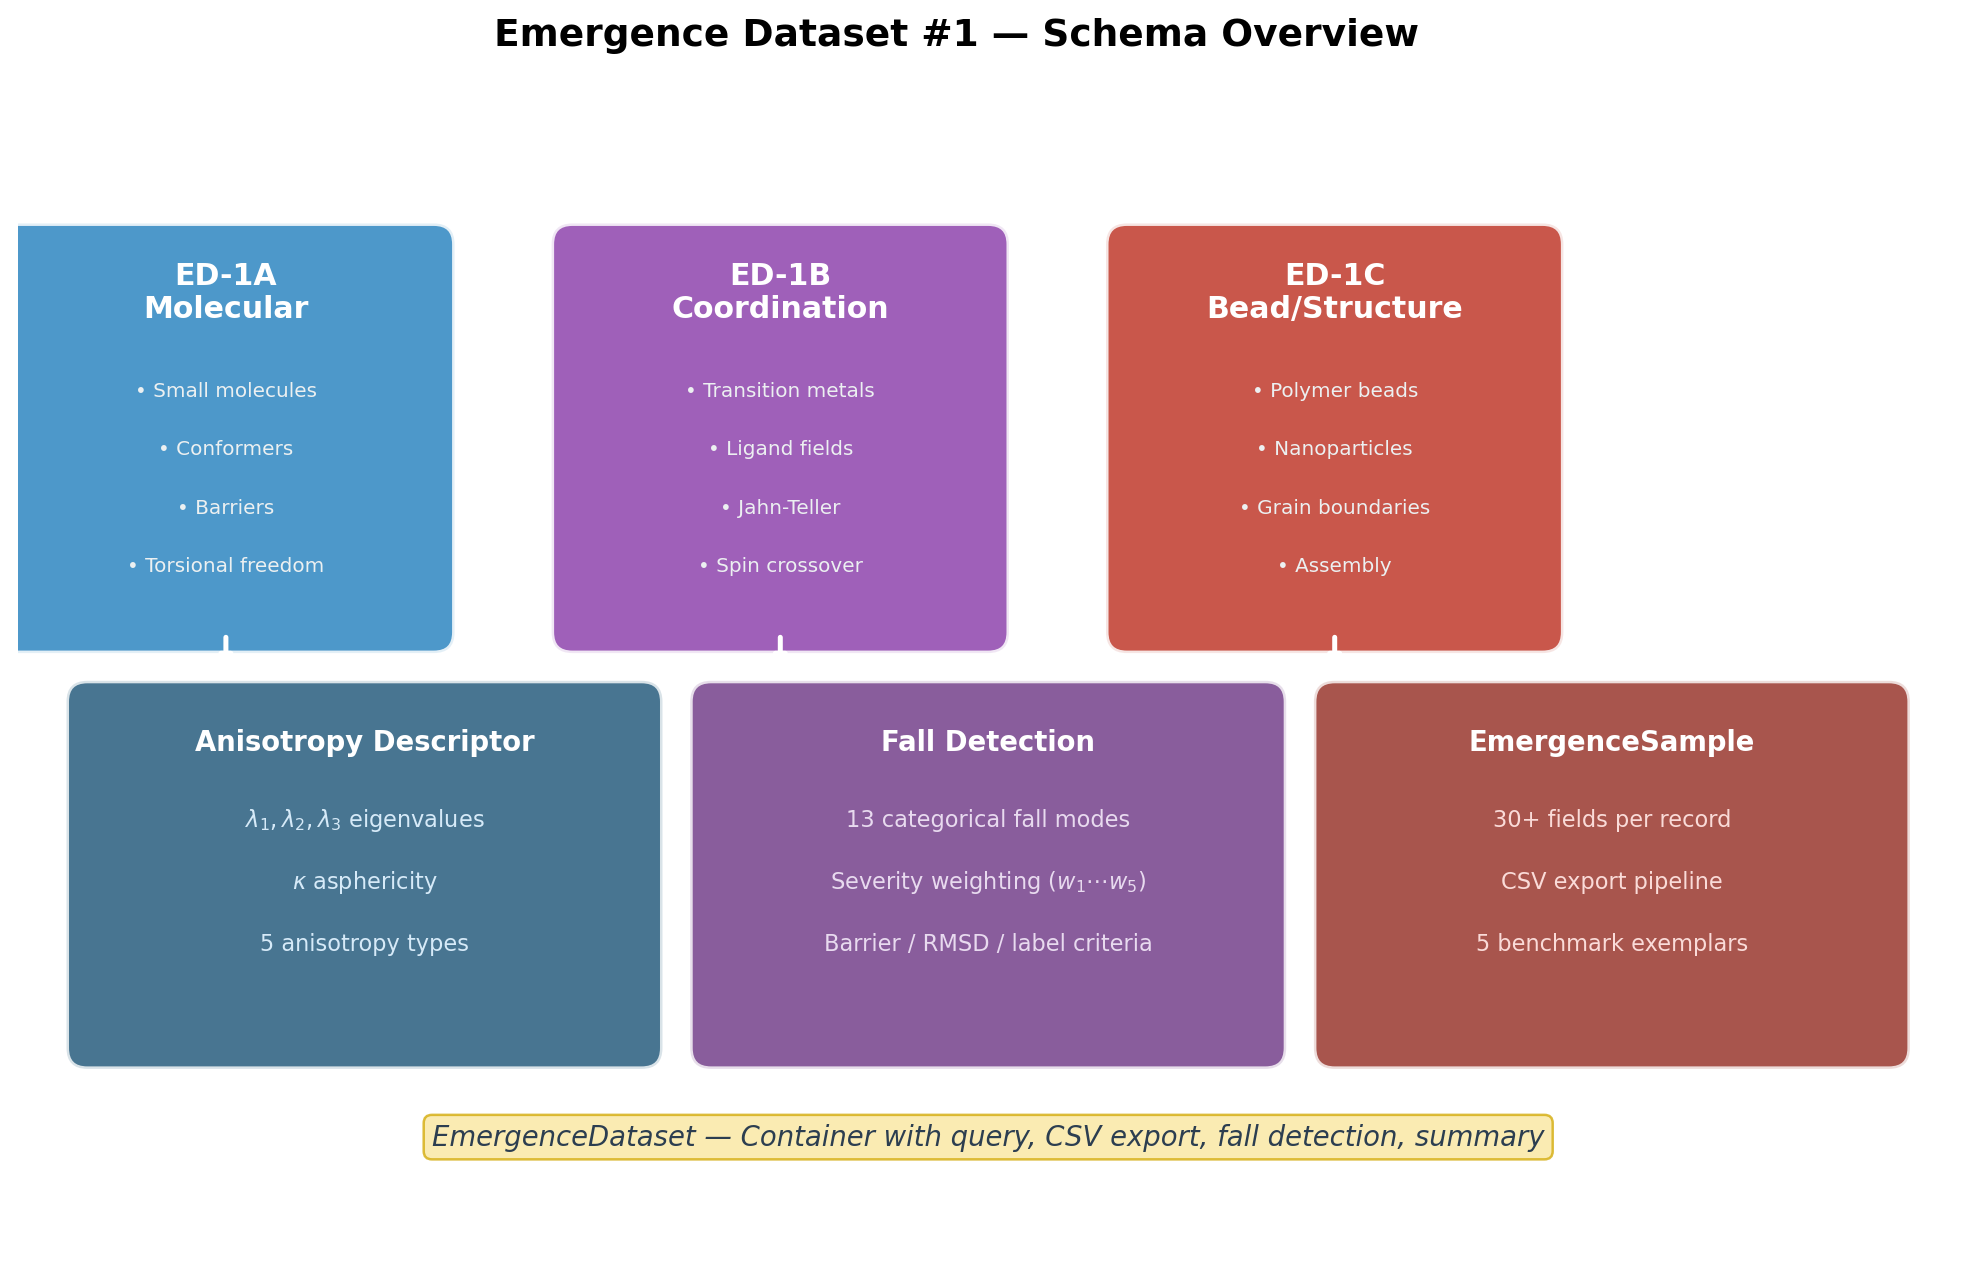
\includegraphics[width=0.85\textwidth]{overview_emergence_schema.png}
\caption{%
	\vsim{} emergence schema: material behavior arises from state
	perturbation and trajectory analysis, not from pre-assigned labels.}
\label{fig:emergence_schema}
\end{figure}

\newpage

% ============================================================
% 2. Universal Simulation Framework
% ============================================================
\section{Universal Simulation Framework}

\subsection{State-History View of Materials}

In \vsim{}, material behavior is treated as a sequence:

\begin{center}
\textbf{Material} $\rightarrow$ \textbf{State} $\rightarrow$
\textbf{Perturbation} $\rightarrow$ \textbf{Trajectory} $\rightarrow$
\textbf{Signature}
\end{center}

Equivalently this project uses the operational pattern:

\begin{center}
\textbf{Initialize} $\rightarrow$ \textbf{Describe} $\rightarrow$
\textbf{Perturb} $\rightarrow$ \textbf{Track} $\rightarrow$ \textbf{Find}
\end{center}

\begin{table}[H]
\centering
\caption{Universal simulation logic.}
\label{tab:sim_logic}
\begin{tabular}{lp{0.35\textwidth}p{0.30\textwidth}}
\toprule
\textbf{Step} & \textbf{Question} & \textbf{Example Output} \\
\midrule
Initialize & What is the starting state? & Chain, lattice, phase, geometry \\
Describe   & What is its structure or topology? & Branching, fibers, domains, defects \\
Perturb    & What physical action is applied? & Heat, compression, defect, shear \\
Track      & What history is recorded? & Positions, displacements, energies \\
Find       & What behavior emerges? & Domain size, anisotropy, diffusion \\
\bottomrule
\end{tabular}
\end{table}

\begin{figure}[H]
\centering
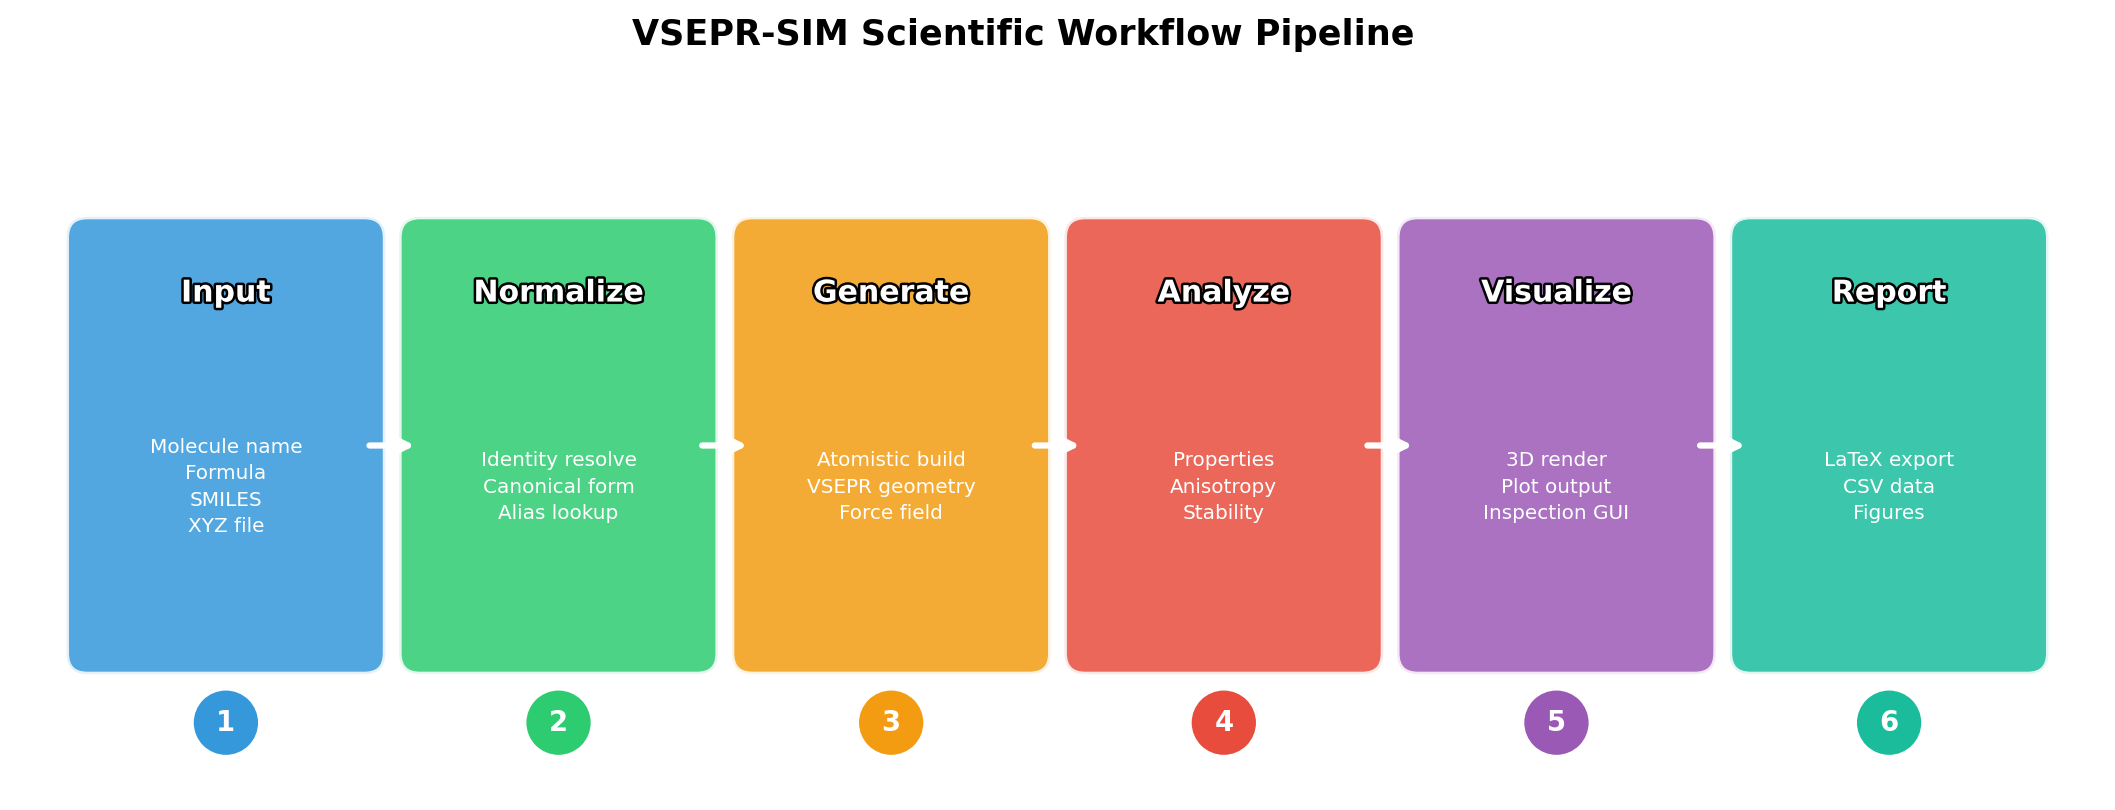
\includegraphics[width=0.82\textwidth]{overview_workflow_pipeline.png}
\caption{%
	\vsim{} workflow pipeline from initialization through report export.
	State files carry only ground-truth history;
	inferred properties live in the analysis layer.}
\label{fig:workflow}
\end{figure}

\subsection{State Files and Artifact Roles}

The project separates state truth, engineering geometry, and analysis outputs.

\begin{table}[H]
\centering
\caption{Artifact roles in the \vsim{} workflow.}
\label{tab:artifacts}
\begin{tabular}{ll}
\toprule
\textbf{Artifact} & \textbf{Role} \\
\midrule
\xyz{}                    & Static particle state \\
\xyzf{}                   & Multi-frame trajectory history \\
\xyzfull{}                & Full replay metadata (positions, velocities, IDs, energy trace) \\
\stepfile{}               & Engineering geometry truth (CAD export artifact) \\
\stlfile{}                & Render, collision, or meshing proxy \\
\texttt{geometry\_map.json} & Binding and provenance map \\
\texttt{analysis.json}    & Derived metrics and inference results \\
\bottomrule
\end{tabular}
\end{table}

\sigbox{%
\textbf{Permanent rule:}
The state file records ground-truth simulation data.
It must not store inferred macro properties such as stiffness, crystallinity,
softness, brittleness, or domain size.
Those belong in the analysis layer.
Encoding conclusions into state and calling it emergence is just lying
with better formatting.%
}

\subsection{Beta-7 Pipeline}

The beta-7 research pipeline wires the following record chain:

\begin{center}
FormationOutput
$\to$ FingerprintRecord
$\to$ ClusterRecord
$\to$ AnalysisRecord
$\to$ ReportRecord
$\to$ DashboardRecord
\end{center}

\begin{table}[H]
\centering
\caption{Beta-7 pipeline stage outputs.}
\label{tab:pipeline}
\begin{tabular}{lll}
\toprule
\textbf{Stage} & \textbf{Input} & \textbf{Output} \\
\midrule
\texttt{stage\_fingerprint} & FormationRecord & 8-feature vector + topology hash \\
\texttt{stage\_cluster}     & FingerprintRecord & Deterministic cluster ID \\
\texttt{stage\_analysis}    & ClusterRecord + FormationRecord & Stability, packing, motif class \\
\texttt{stage\_report}      & AnalysisRecord & CSV row, JSON fragment, summary \\
\texttt{stage\_dashboard}   & All ReportRecords & Markdown table + JSON array \\
\bottomrule
\end{tabular}
\end{table}

\begin{figure}[H]
\centering
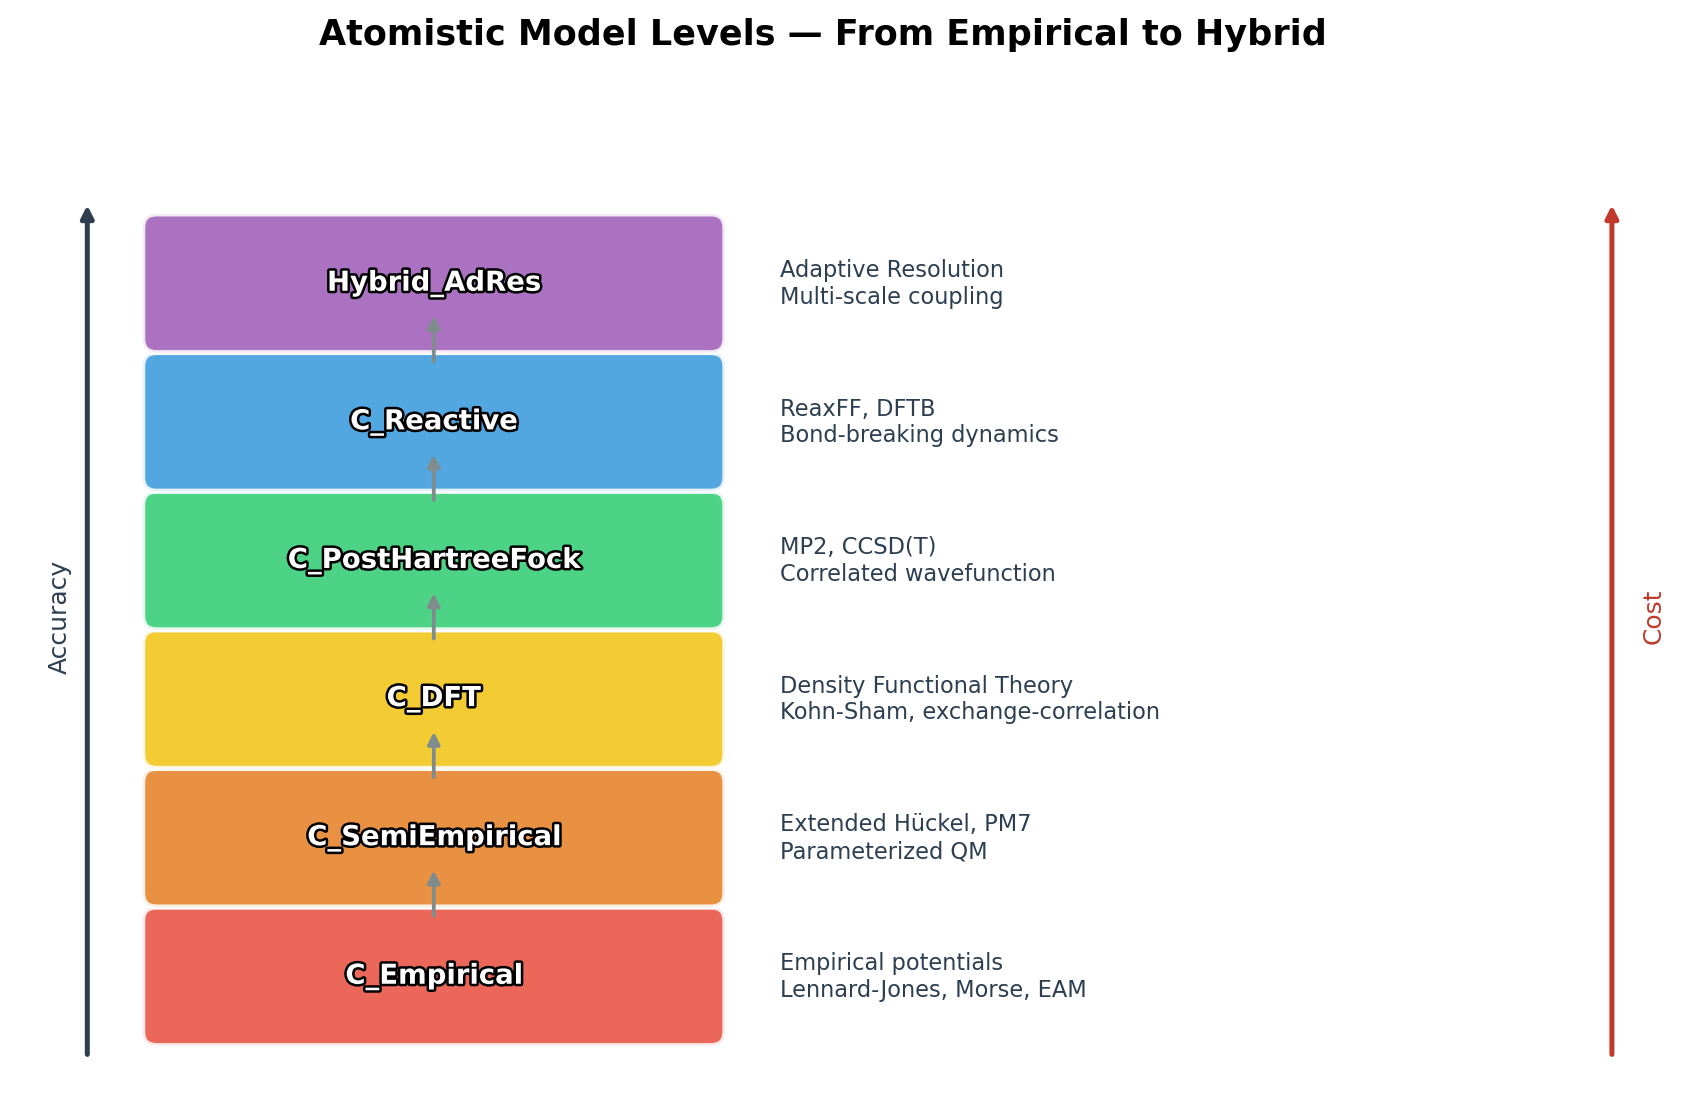
\includegraphics[width=0.80\textwidth]{overview_model_levels.png}
\caption{%
	\vsim{} model levels from atomistic through coarse-grained to
	premacro and macro inference layers.}
\label{fig:model_levels}
\end{figure}

\subsection{Scale Registry}

\begin{table}[H]
\centering
\caption{Simulation scale registry.}
\label{tab:scales}
\begin{tabular}{lllll}
\toprule
\textbf{Scale} & \textbf{Name} & \textbf{Length} & \textbf{Time} & \textbf{Status} \\
\midrule
1 & Atomistic     & \si{\angstrom} & \si{fs}  & Active \\
2 & Coarse-grained & nm            & ps       & Active \\
3 & Grain / microstructure & \si{\micro m} & ns & Partial \\
4 & Component     & mm            & \si{\micro s} & Planned \\
5 & Macroscopic   & m             & s        & Planned \\
\bottomrule
\end{tabular}
\end{table}

\newpage

% ============================================================
% 3. Universal Smoke Tests
% ============================================================
\section{Universal Smoke-Test Gate}
\label{sec:smoketests}

Before any material result is accepted, the simulation must pass a universal
smoke-test gate confirming that the system can initialize, run, record, analyze,
validate, and report without silent failure.

\subsection{CLI and Scripting Tests}

\begin{table}[H]
\centering
\caption{Mundane but necessary CLI tests.}
\label{tab:cli_tests}
\begin{tabular}{lll}
\toprule
\textbf{Test} & \textbf{Command} & \textbf{Pass Condition} \\
\midrule
Help/version   & \texttt{vsper --help}             & Commands print correctly \\
Version        & \texttt{vsper --version}           & Version recorded \\
Script parse   & \texttt{vsper validate script.vsim}& Errors show line numbers \\
Minimal run    & \texttt{vsper run smoke.vsim}      & State, trajectory, report created \\
Reproducibility & Same seed twice                   & Same output within tolerance \\
\bottomrule
\end{tabular}
\end{table}

\subsection{State and Trajectory Integrity}

Every state and trajectory file must satisfy:

\begin{itemize}[noitemsep]
	\item valid particle count,
	\item finite coordinates,
	\item no missing persistent IDs,
	\item no duplicate IDs unless event-logged,
	\item monotonic time steps,
	\item stable particle identity across frames,
	\item no inferred macro properties stored in state files.
\end{itemize}

\subsection{Universal Analysis Tests}

\begin{table}[H]
\centering
\caption{Universal analysis smoke tests.}
\label{tab:analysis_smoke}
\begin{tabular}{lp{0.50\textwidth}}
\toprule
\textbf{Analysis} & \textbf{Purpose} \\
\midrule
RMSD / displacement      & Detect deformation and motion \\
Cluster/domain detection & Measure emergent structures \\
Local order              & Identify packing, coordination, alignment \\
Diffusion / mobility     & Estimate movement and transport \\
Packing / porosity       & Estimate free volume and density trends \\
Anisotropy               & Detect directional behavior \\
Report export            & Verify reproducible documentation \\
\bottomrule
\end{tabular}
\end{table}

\subsection{Beta-7 Pipeline Smoke Test Results}

The beta-7 pipeline was validated on the 12-element metallic reference dataset.

\begin{table}[H]
\centering
\caption{Beta-7 pipeline smoke-test results (12-element reference).}
\label{tab:pipeline_smoke}
\begin{tabular}{lrrll}
\toprule
\textbf{Element} & \textbf{Stability} & \textbf{Pack} & \textbf{Cluster} & \textbf{Warnings} \\
\midrule
Au (Gold)        & 0.584 & 0.430 & FCC-sparse & low\_population \\
Ag (Silver)      & 0.700 & 0.000 & FCC-sparse & low\_population \\
Cu (Copper)      & 0.700 & 0.000 & FCC-sparse & --- \\
Pt (Platinum)    & 0.000 & 0.000 & FCC-sparse & not\_converged \\
Ni (Nickel)      & 0.000 & 0.000 & FCC-sparse & not\_converged \\
Al (Aluminium)   & 0.699 & 0.000 & FCC-sparse & --- \\
Fe (Iron)        & 0.652 & 0.847 & BCC-dense  & low\_population \\
W  (Tungsten)    & 0.612 & 0.714 & BCC-dense  & low\_population \\
Mo (Molybdenum)  & 0.617 & 0.721 & BCC-dense  & low\_population \\
Cr (Chromium)    & 0.648 & 0.839 & BCC-dense  & low\_population \\
Ti (Titanium)    & 0.699 & 0.000 & HCP-sparse & low\_population \\
Co (Cobalt)      & 0.044 & 0.000 & HCP-sparse & not\_converged \\
\bottomrule
\end{tabular}
\end{table}

All 377 assertions passed (T1--T8).
Cluster assignment is deterministic across runs.
BCC-dense metals (Fe, W, Mo, Cr) correctly group by high packing quality.
Low-population warnings appear because the 12-element set is a single-instance
reference; they are expected and non-fatal.

\subsection{Emergence Validation Rule}

A result counts as emergent only if the measured feature is \emph{produced}
by the run and \emph{detected} afterward.

\begin{equation}
	\epsilon = \frac{|D_{\mathrm{sim}} - D_{\mathrm{expected}}|}{D_{\mathrm{expected}}}
	\label{eq:epsilon}
\end{equation}

For morphology targets such as polyethylene domain size the preliminary
acceptance criterion is:

\begin{equation}
	\epsilon \leq 0.20
	\label{eq:acceptance}
\end{equation}

\begin{figure}[H]
\centering
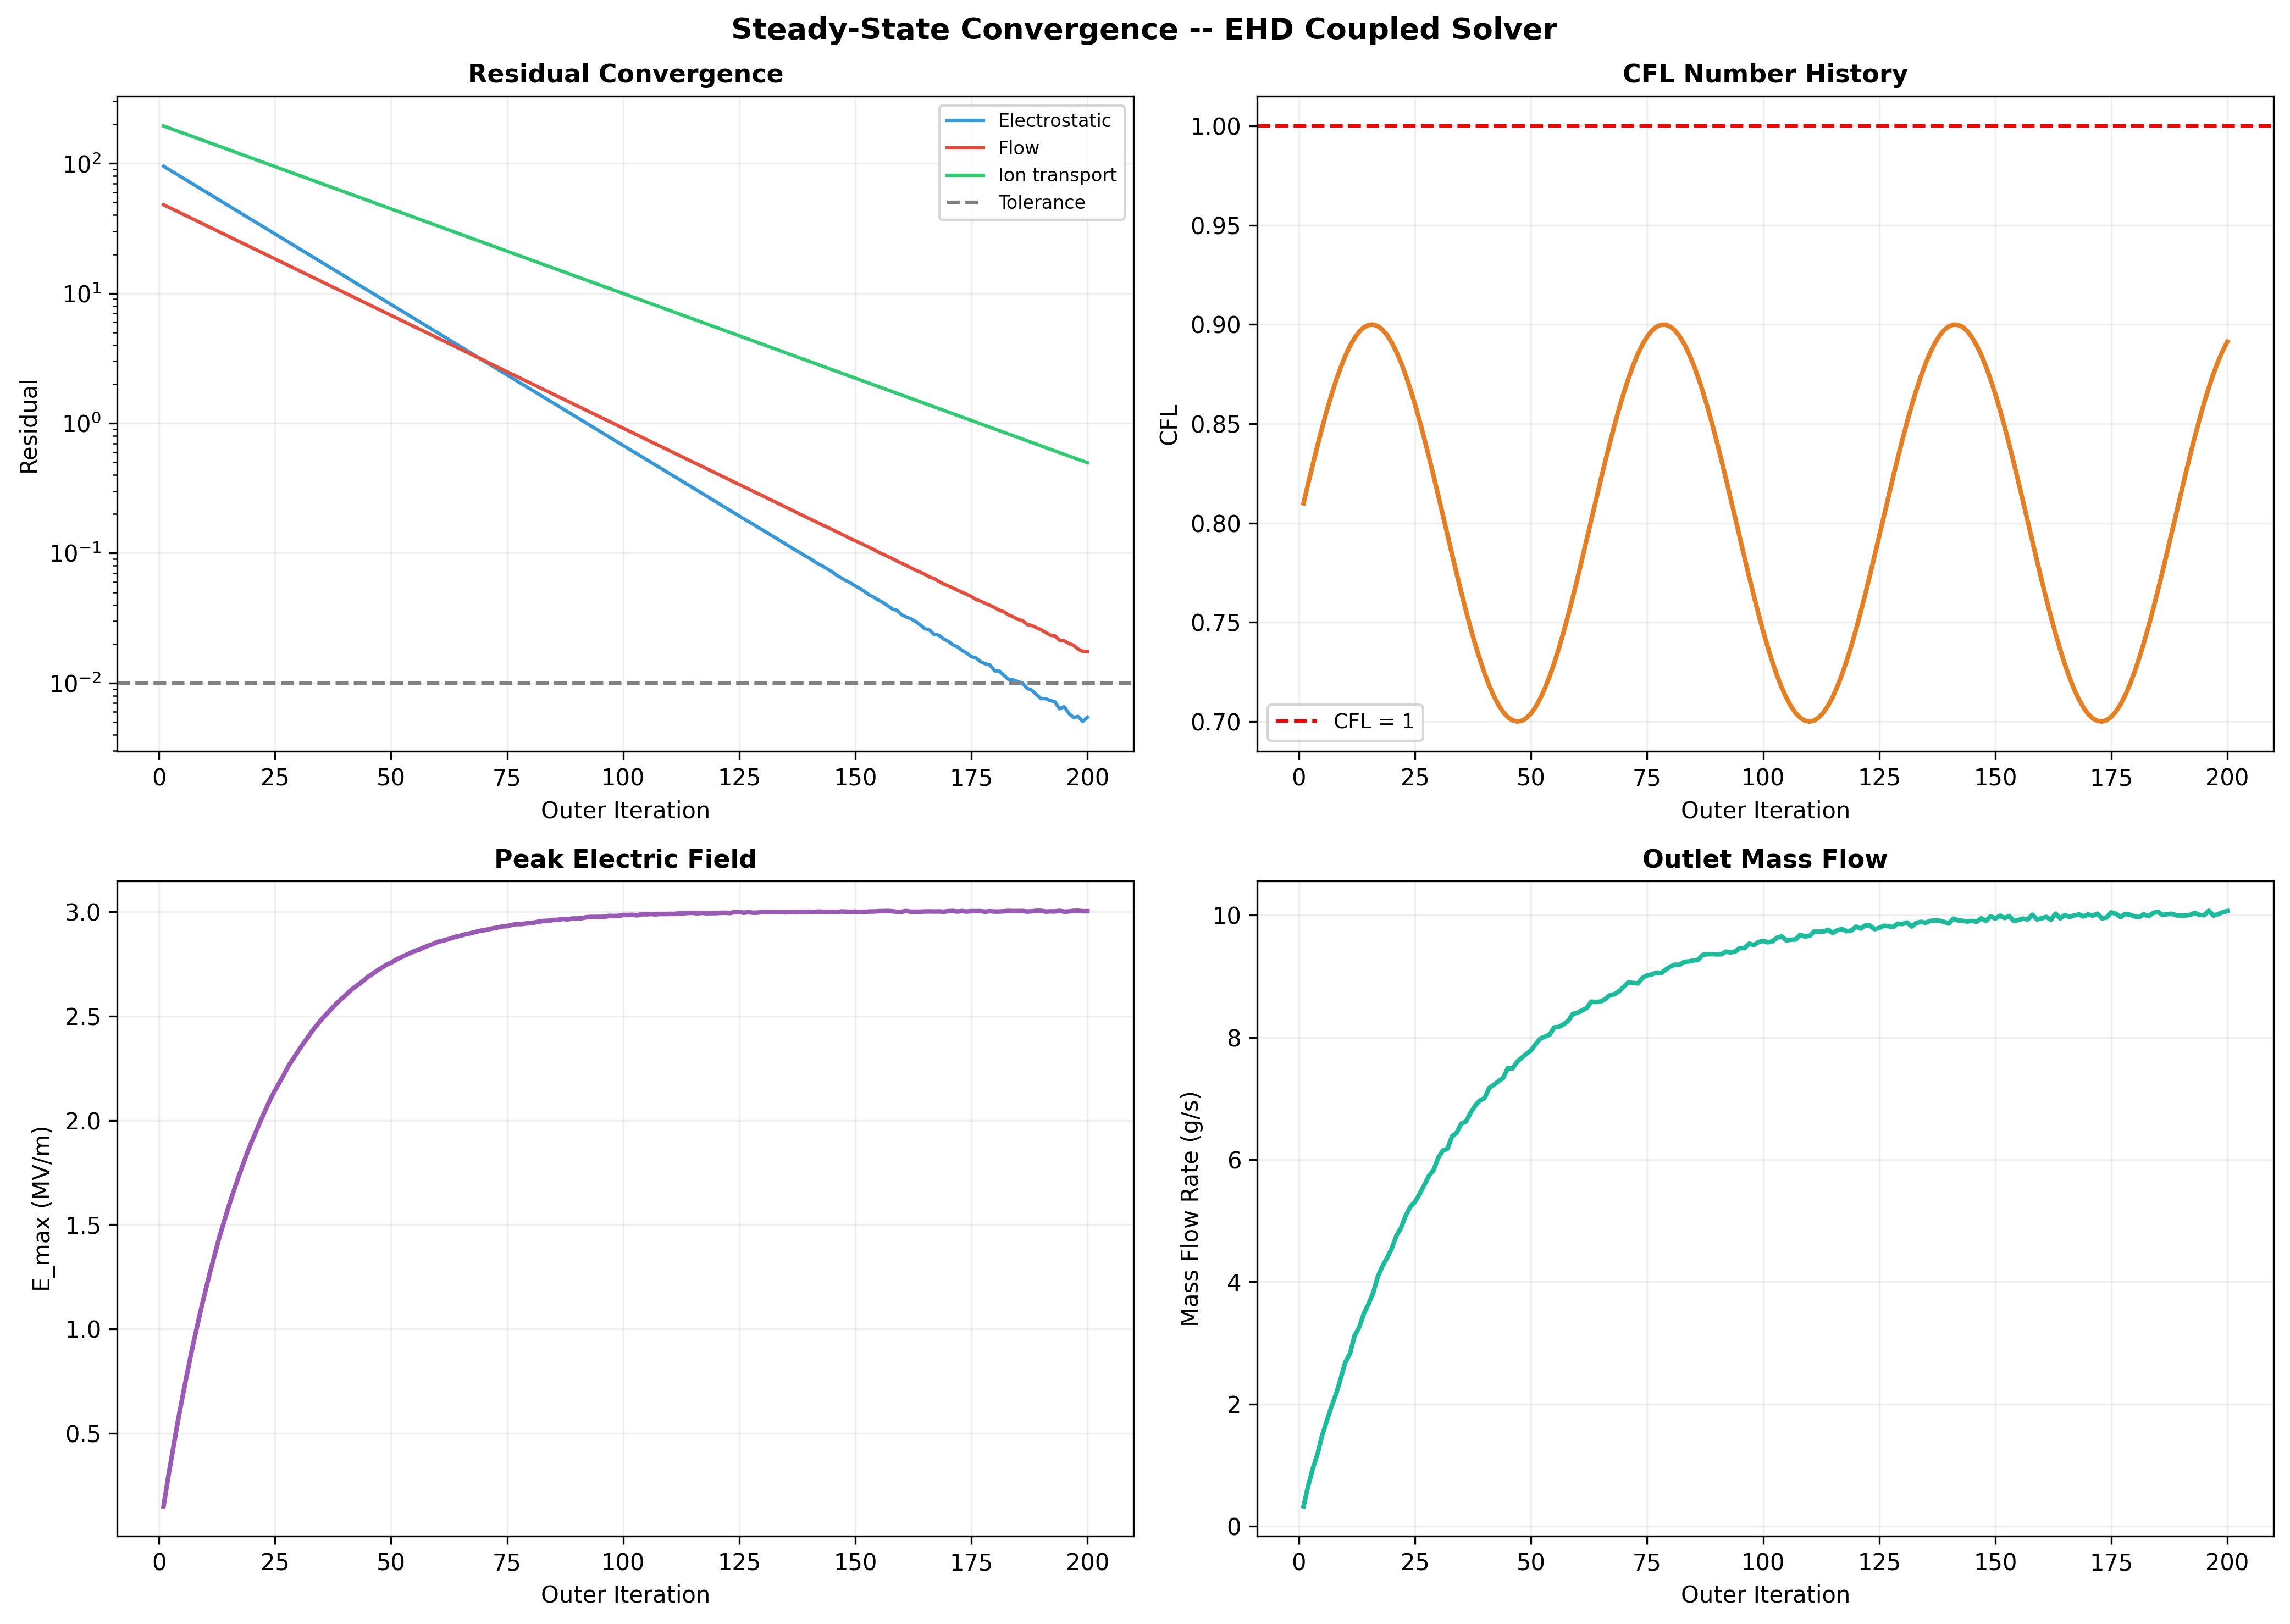
\includegraphics[width=0.72\textwidth]{steady_state_convergence.png}
\caption{%
	Convergence indicator during formation run.
	Stationarity is determined by \texttt{StationarityGate}
	(relative drift criterion); measurements begin only after the gate
	opens.}
\label{fig:convergence}
\end{figure}

\newpage

% ============================================================
% 4. Material Set Overview
% ============================================================
\section{Material Set Overview}

The fifteen materials span conventional and advanced material classes.

\begin{longtable}{p{0.05\textwidth}p{0.22\textwidth}p{0.22\textwidth}p{0.38\textwidth}}
\caption{Fifteen-material review set.}
\label{tab:material_set}\\
\toprule
\textbf{\#} & \textbf{Material} & \textbf{Class} & \textbf{Primary Signature} \\
\midrule
\endfirsthead
\toprule
\textbf{\#} & \textbf{Material} & \textbf{Class} & \textbf{Primary Signature} \\
\midrule
\endhead
1  & Aluminum             & Metal                  & Ductile recovery and defect tolerance \\
2  & Alumina              & Ceramic                & Rigidity until failure \\
3  & Polyethylene         & Polymer                & Chain topology becoming macro behavior \\
4  & Carbon fiber epoxy   & Composite              & Architecture becoming directional behavior \\
5  & Silicon              & Semiconductor          & Defect-sensitive covalent order \\
6  & Naphthalene / PAH    & Exotic hydrocarbon     & Aromatic structure becoming carbon behavior \\
7  & Argon / Xenon        & Noble material         & Phase behavior with minimal chemistry \\
8  & Fe-Cr-Ni alloy       & Irradiated alloy       & Damage history becoming material history \\
9  & Hexene               & Organic chain          & Small-molecule chain flexibility \\
10 & Cyclopentadiene      & Ring ligand proxy      & Geometry-sensitive interaction \\
11 & Graphite / graphene  & Layered carbon         & Anisotropy from layered structure \\
12 & FLiBe proxy          & Molten salt            & Ionic transport as structure \\
13 & Tungsten alloy       & Refractory metal       & High-temperature structural persistence \\
14 & PDMS                 & Elastomer              & Soft deformation with recovery \\
15 & Zircaloy proxy       & Nuclear alloy          & Surface degradation and radiation memory \\
\bottomrule
\end{longtable}

\begin{figure}[H]
\centering
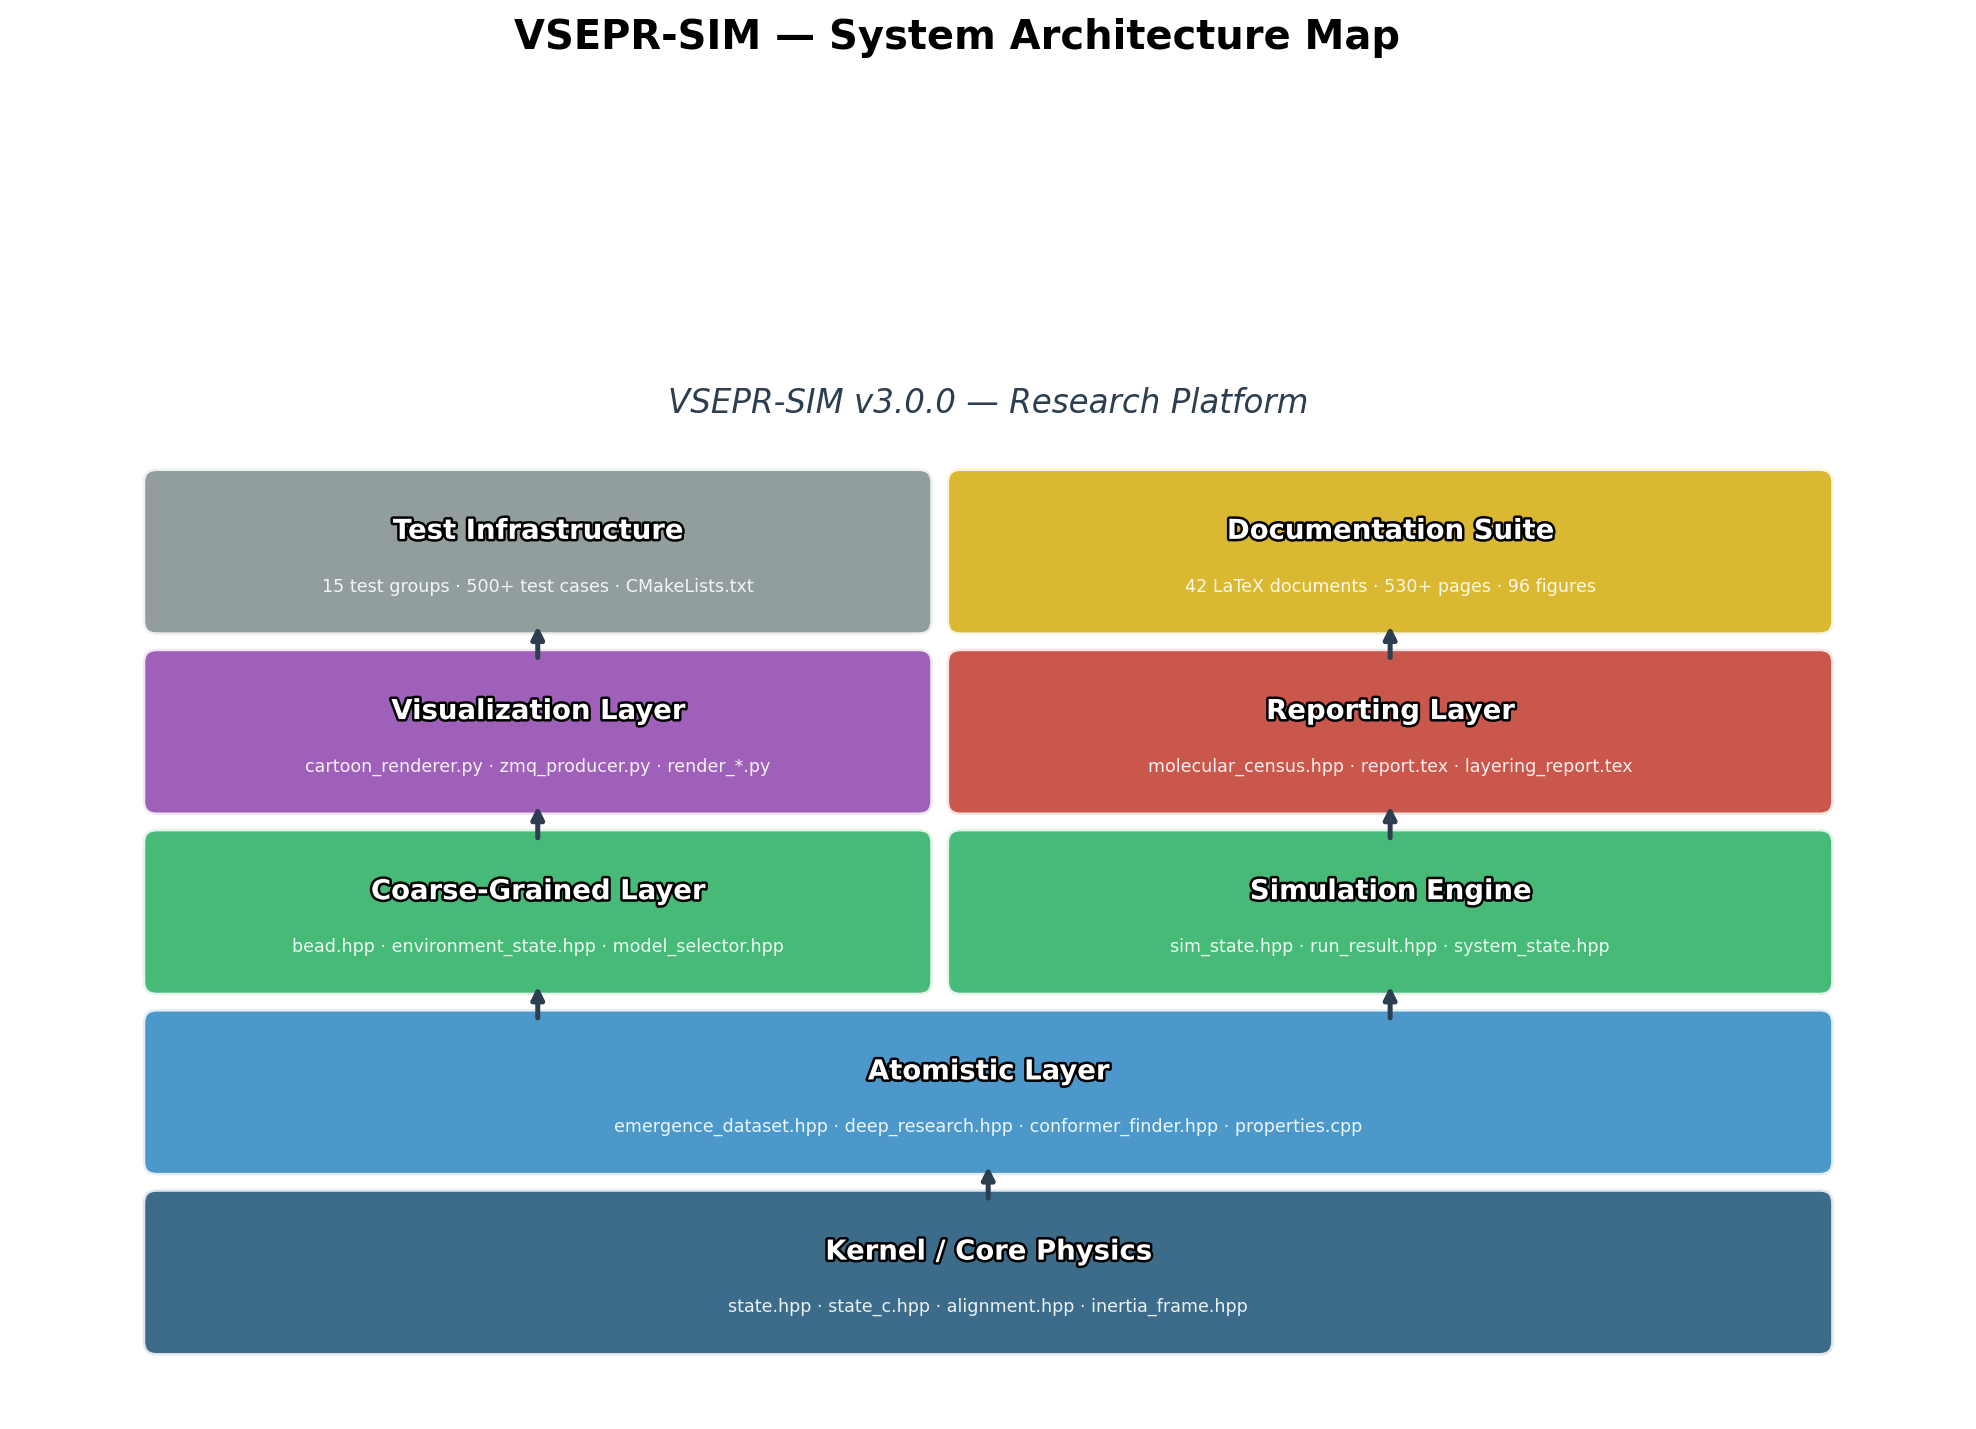
\includegraphics[width=0.80\textwidth]{overview_architecture_map.png}
\caption{%
	Architecture map locating each material class within the
	\vsim{} scale and analysis hierarchy.}
\label{fig:arch_map}
\end{figure}

\newpage

% ============================================================
% 5. Material Cards
% ============================================================
\section{Material Cards}

% ============================================================
% Card 01 --- Aluminum
% ============================================================
\cardheader{Card~01 --- Aluminum}{Metal}%
{Lightweight heat-transfer bracket or duct support under vibration and thermal cycling}

\textbf{\vsim{} role:} Ductile crystalline metal baseline.

\begin{figure}[H]
\centering
\begin{subfigure}[b]{0.46\textwidth}
	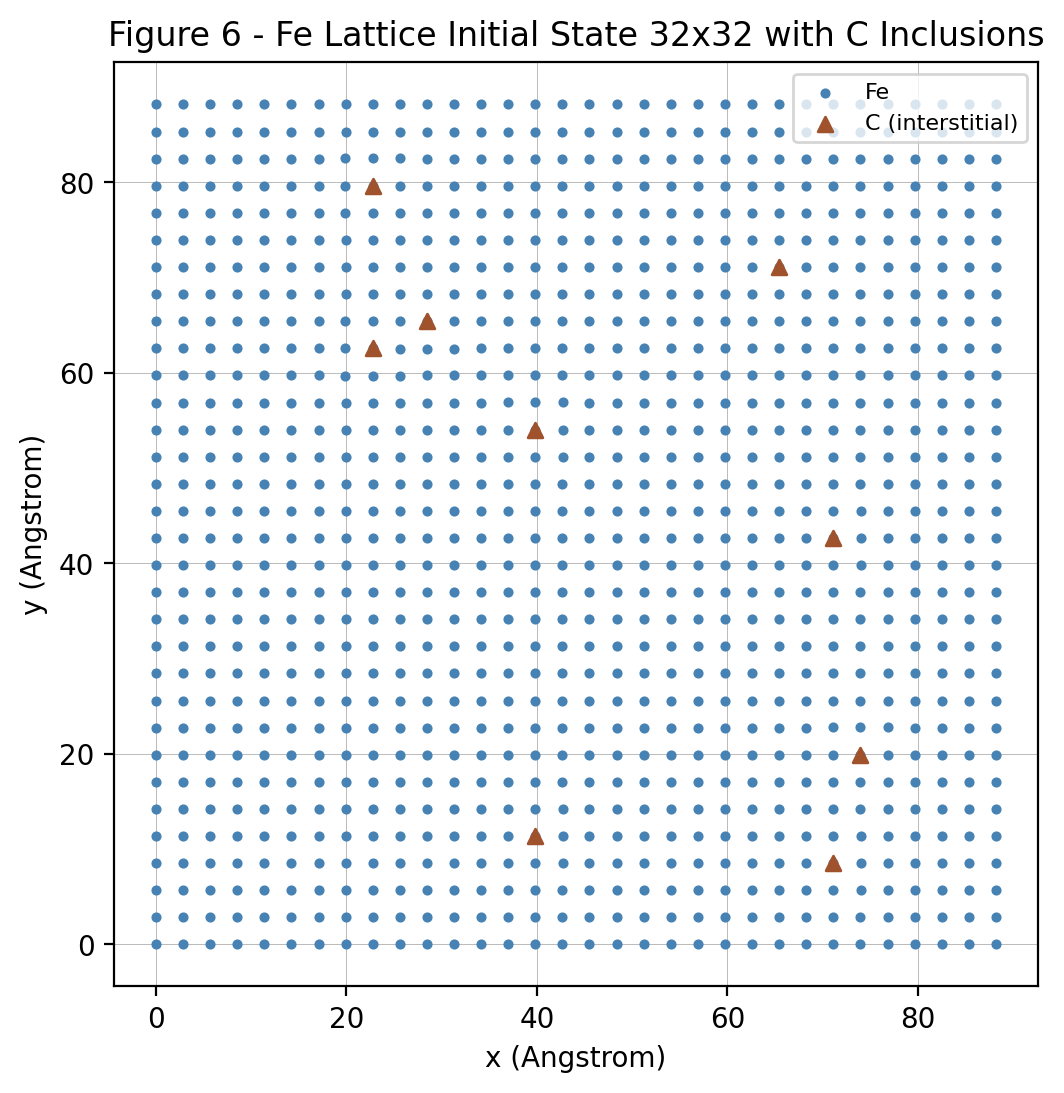
\includegraphics[width=\textwidth]{fig6_lattice_initial.png}
	\caption{FCC lattice --- initial state.}
\end{subfigure}
\hfill
\begin{subfigure}[b]{0.46\textwidth}
	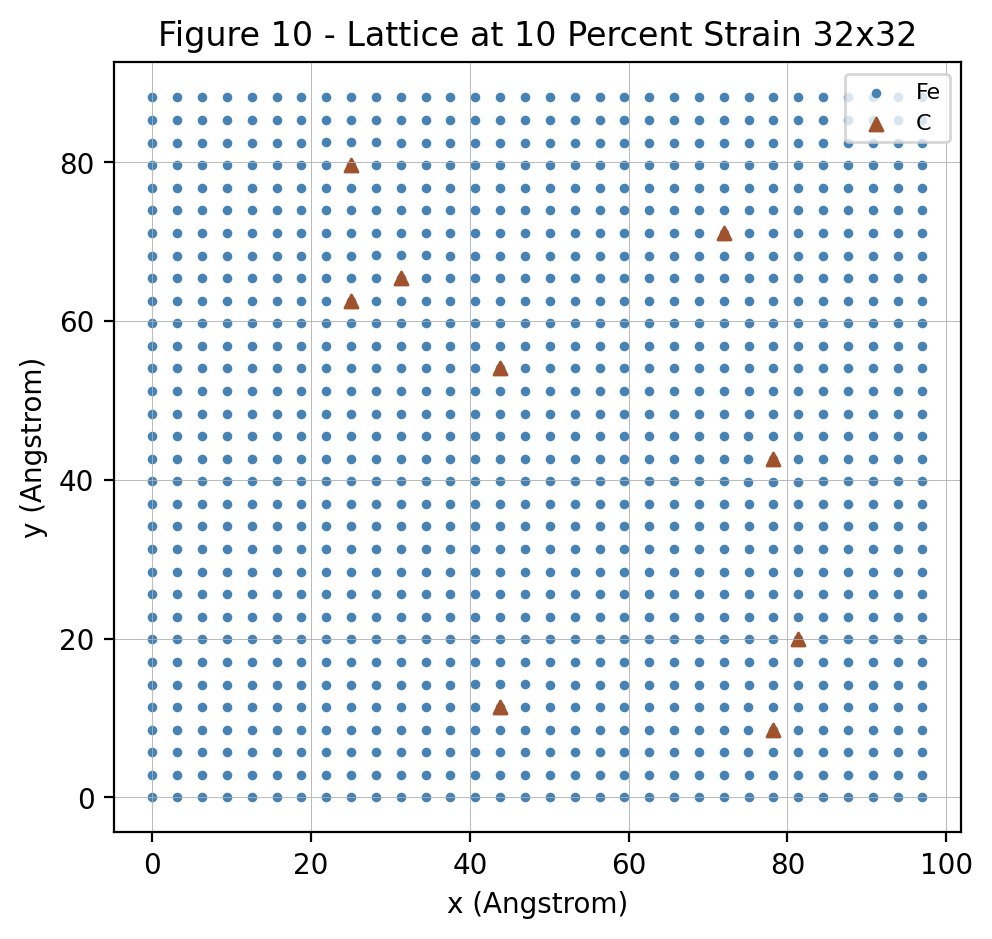
\includegraphics[width=\textwidth]{fig10_lattice_deformed.png}
	\caption{Lattice after defect perturbation.}
\end{subfigure}
\caption{%
	Aluminum FCC lattice before and after vacancy injection.
	RMSD and coordination change are the primary diagnostic outputs.}
\label{fig:al_lattice}
\end{figure}

\begin{figure}[H]
\centering
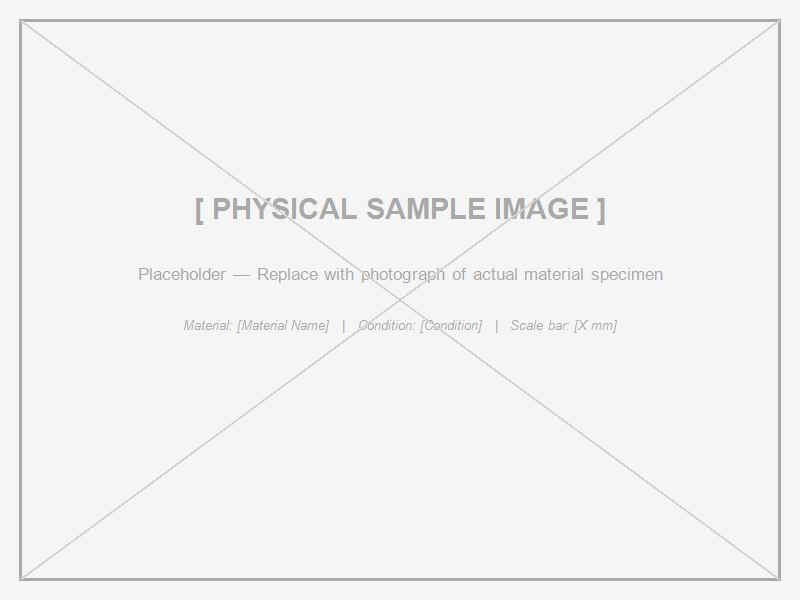
\includegraphics[width=0.55\textwidth]{sample_placeholder.png}
\caption{%
	\textbf{Physical sample placeholder.}
	Replace with photograph of an aluminum alloy specimen
	(e.g., 6061-T6 coupon, grain-etched cross-section, or fractured surface).
	Scale bar should indicate grain size range.}
\label{fig:al_sample}
\end{figure}

\textbf{Simulation tests:}
\begin{itemize}[noitemsep]
	\item FCC lattice initialization,
	\item vacancy and interstitial defects,
	\item thermal jitter at elevated temperature,
	\item localized impulse,
	\item relaxation tracking.
\end{itemize}

\textbf{Recorded signatures:}
\begin{itemize}[noitemsep]
	\item RMSD from ideal lattice,
	\item defect fraction,
	\item coordination change,
	\item relaxation time,
	\item crystal persistence.
\end{itemize}

\textbf{Pipeline result from reference dataset (Al):}
Stability score~$= 0.699$, cluster assignment FCC-sparse,
energy per bead $= \num{-0.000012}$~kcal/mol,
convergence quality~$= 0.699$.
Formation converged in 5~FIRE steps.

\materialsignature{Aluminum's signature is defect tolerance through ductile recovery.}

% ============================================================
% Card 02 --- Alumina
% ============================================================
\cardheader{Card~02 --- Alumina}{Ceramic}%
{High-temperature ceramic liner or electrical insulation tile}

\textbf{\vsim{} role:} Brittle high-stability ceramic baseline.

\textbf{Simulation tests:}
\begin{itemize}[noitemsep]
	\item ordered oxide lattice proxy,
	\item thermal impulse,
	\item vacancy defect,
	\item crack-seed perturbation,
	\item low-diffusion tracking.
\end{itemize}

\textbf{Recorded signatures:}
\begin{itemize}[noitemsep]
	\item localized damage persistence,
	\item low diffusion proxy,
	\item poor defect recovery,
	\item structural persistence.
\end{itemize}

\begin{figure}[H]
\centering
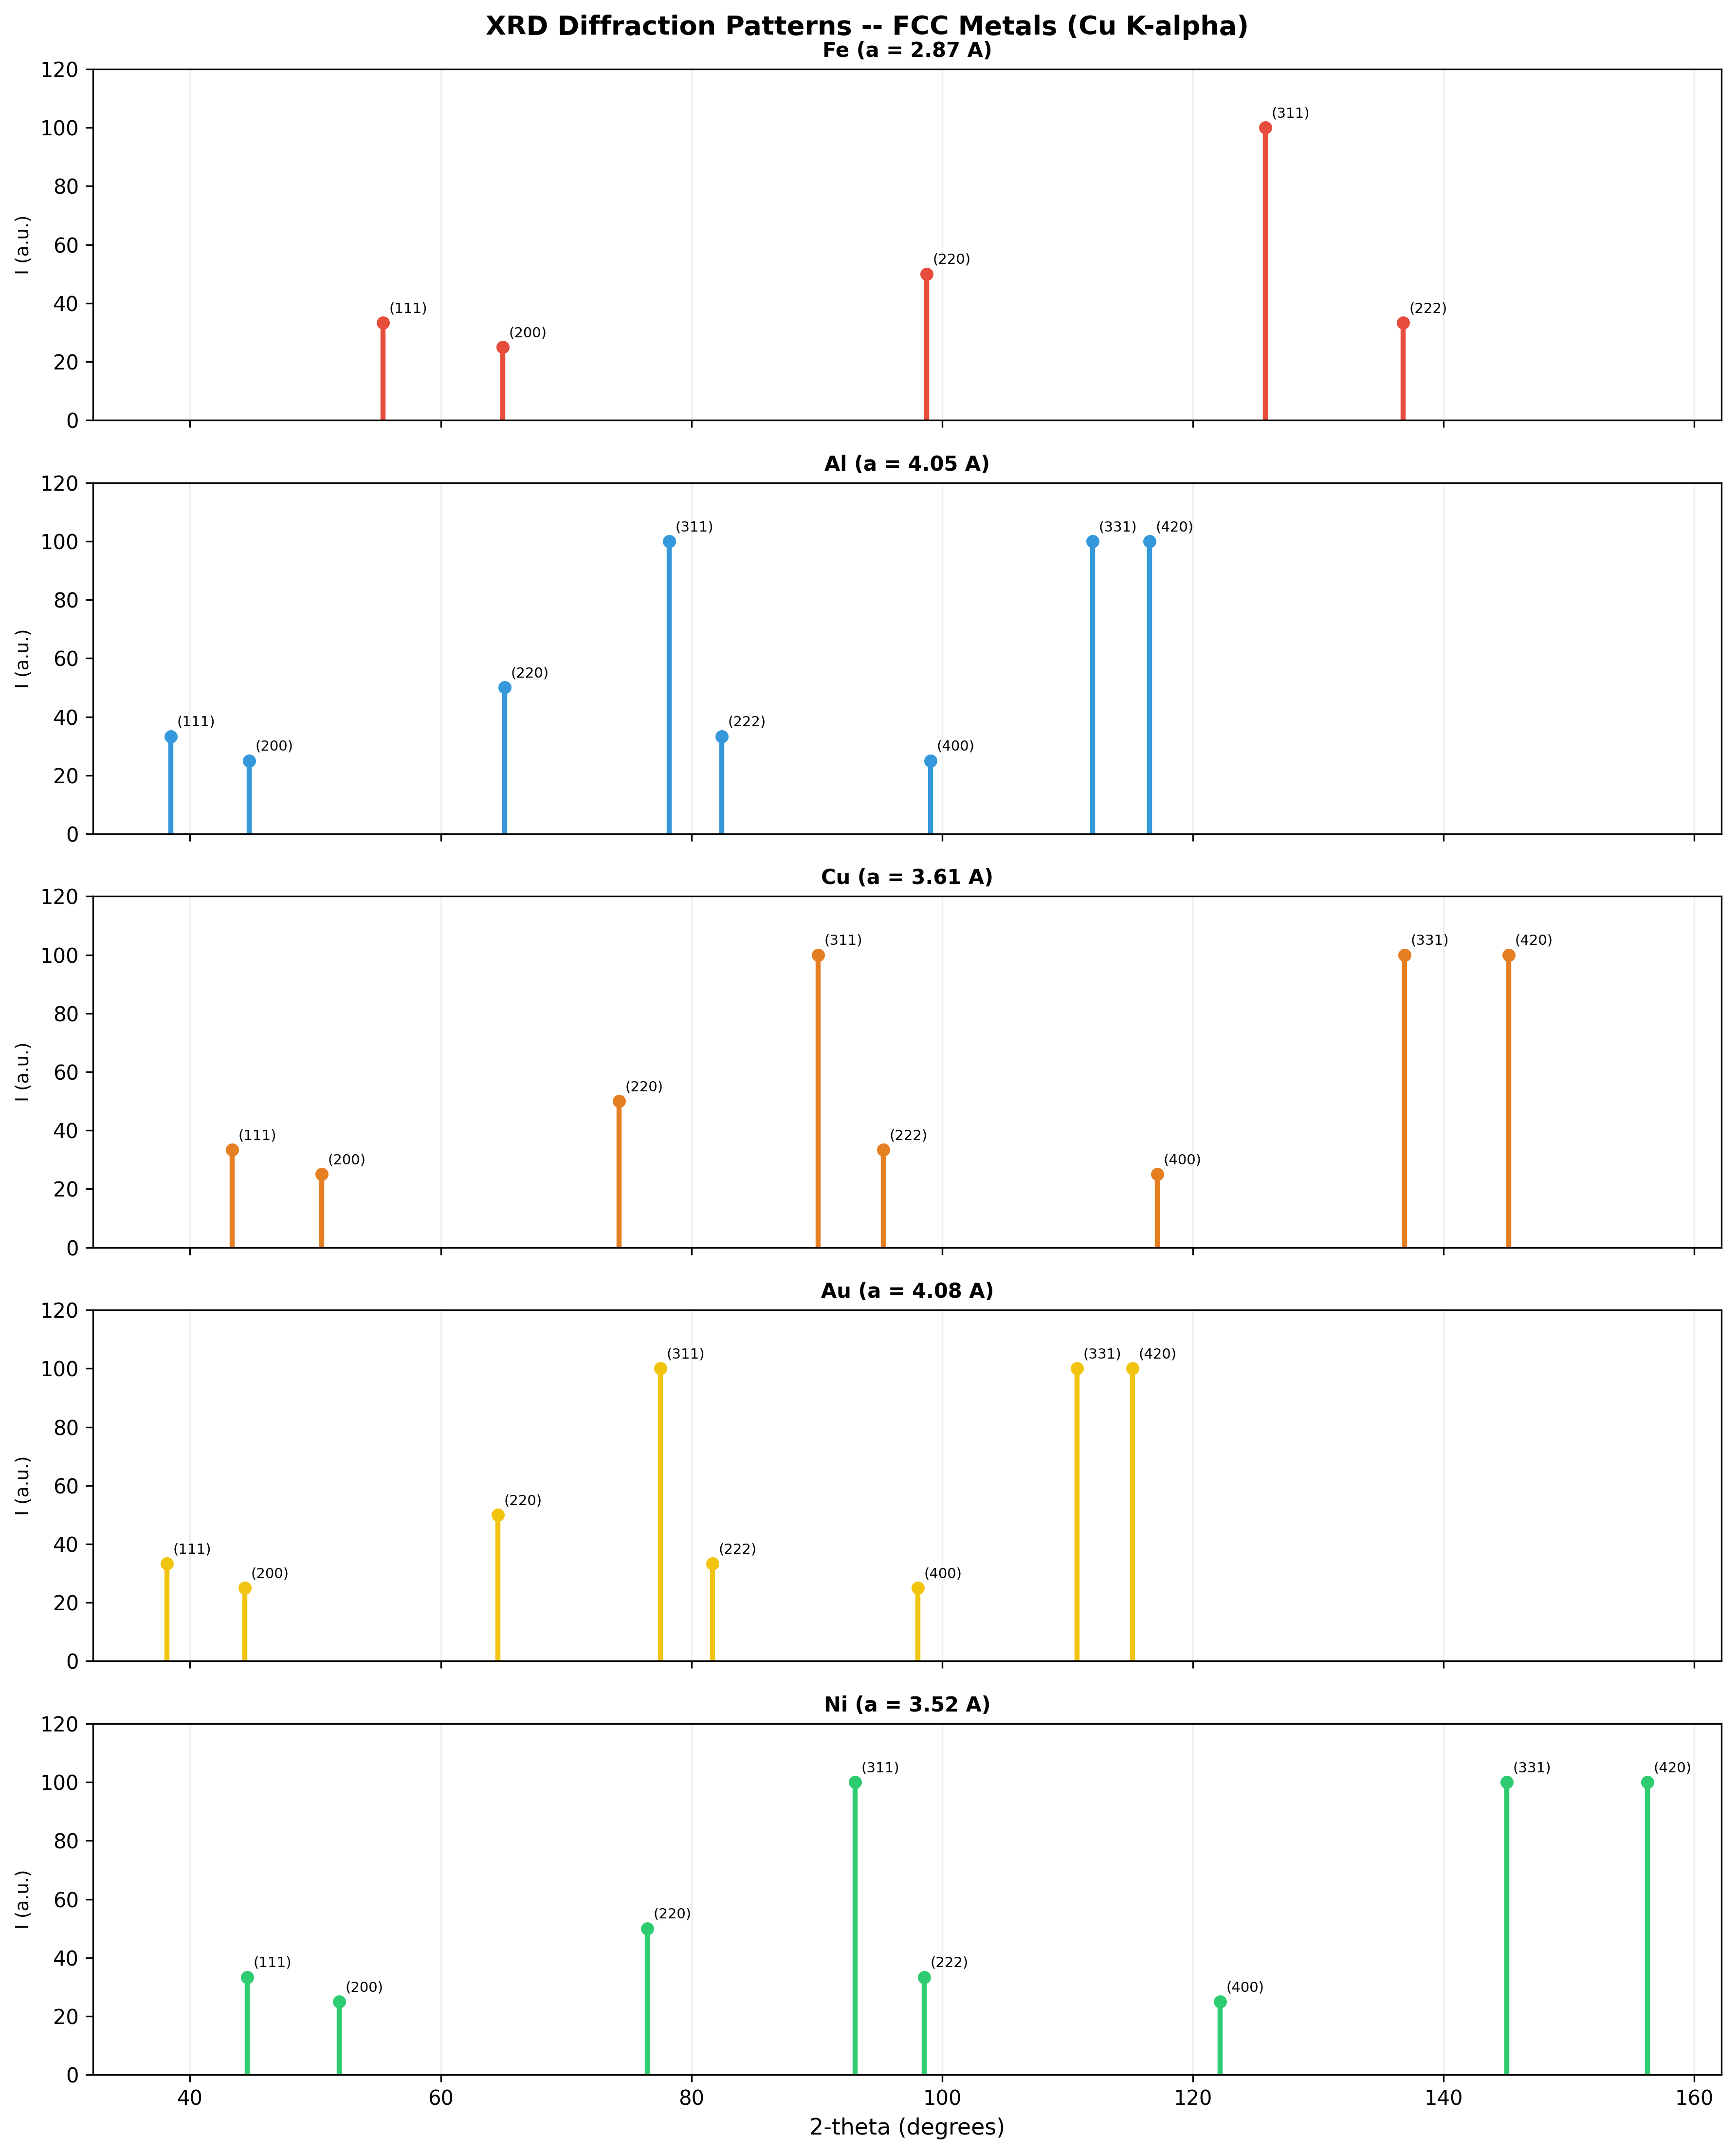
\includegraphics[width=0.55\textwidth]{xrd_patterns.png}
\caption{%
	Representative XRD pattern proxy.
	For alumina, the diffraction peaks are sharp and stable,
	consistent with a well-ordered oxide lattice.
	Defect perturbation broadens peaks and shifts positions.}
\label{fig:alumina_xrd}
\end{figure}

\materialsignature{Alumina's signature is rigidity until failure.}

\newpage

% ============================================================
% Card 03 --- Polyethylene (Expanded)
% ============================================================
\cardheader{Card~03 --- Polyethylene (Expanded)}{Polymer}%
{Flexible seal, low-friction liner, compressible polymer interface, or packaging film proxy}

\subsubsection*{Material Overview}

Polyethylene is a chain-based polymer with repeat unit:

\begin{equation}
	[-\mathrm{CH}_2\text{--}\mathrm{CH}_2-]_n
	\label{eq:pe_repeat}
\end{equation}

Its macro behavior depends strongly on chain length, branching, packing,
and thermal motion.
Unlike a perfect crystal, polyethylene is best understood through chain topology
and morphology, making it an ideal test case for \vsim{}:
the most important result must emerge from formation mechanics rather than be
assigned directly.

\materialsignature{%
Polyethylene's signature is chain topology becoming macro behavior.%
}

\subsubsection*{Variants}

\begin{table}[H]
\centering
\caption{Polyethylene family variants.}
\label{tab:pe_variants}
\begin{tabular}{lll}
\toprule
\textbf{Variant} & \textbf{Structure} & \textbf{Purpose} \\
\midrule
HDPE proxy & Mostly linear PE chains   & High-packing baseline \\
LDPE proxy & Branched PE chains        & Disrupted-packing comparison \\
PP comparator & Methyl side groups     & Side-group steric comparison \\
\bottomrule
\end{tabular}
\end{table}

\subsubsection*{Primary Emergent Variable}

The primary emergent variable is the average locally ordered polymer domain size
$D_{\mathrm{domain,avg}}$.
This is not an input.
It is measured after the run using chain alignment, packing density,
local order, neighbor connectivity, and residence stability.

\subsubsection*{Formation Pipeline}

\begin{enumerate}[noitemsep]
	\item Initialize random polymer chains.
	\item Apply melt-like thermal disorder.
	\item Cool or relax the system.
	\item Allow chains to pack, align, and cluster.
	\item Detect locally ordered domains.
	\item Measure domain-size distribution.
	\item Compare simulated average domain size to expected value.
\end{enumerate}

\subsubsection*{Simulation Tests}

\begin{table}[H]
\centering
\caption{Polyethylene simulation tests.}
\label{tab:pe_tests}
\begin{tabular}{ll}
\toprule
\textbf{Test} & \textbf{Purpose} \\
\midrule
Chain packing relaxation & Measure packing fraction and free volume \\
Compression and release  & Measure recovery and hysteresis proxy \\
Thermal motion           & Measure softening and segment mobility \\
Chain stretching         & Measure orientation and end-to-end response \\
Surface contact          & Measure sealing/contact behavior \\
\bottomrule
\end{tabular}
\end{table}

\subsubsection*{Metrics}

\begin{table}[H]
\centering
\caption{Polyethylene metrics.}
\label{tab:pe_metrics}
\begin{tabular}{ll}
\toprule
\textbf{Metric} & \textbf{Meaning} \\
\midrule
$R_g$                      & Radius of gyration \\
$R_e$                      & End-to-end distance \\
$D_{\mathrm{domain,avg}}$  & Average ordered-domain size \\
Packing fraction           & Occupied volume proxy \\
Porosity proxy             & Free-volume estimate \\
Relaxation time            & Recovery after perturbation \\
Orientation parameter      & Chain alignment \\
Hysteresis proxy           & Unrecovered deformation \\
\bottomrule
\end{tabular}
\end{table}

\subsubsection*{Expected Trends}

\begin{table}[H]
\centering
\caption{Expected polyethylene-family trends.}
\label{tab:pe_trends}
\begin{tabular}{p{0.18\textwidth}p{0.32\textwidth}p{0.34\textwidth}}
\toprule
\textbf{Variant} & \textbf{Expected Signature} & \textbf{Macro Interpretation} \\
\midrule
HDPE & Higher packing, larger ordered domains & Higher stiffness and density trend \\
LDPE & Higher free volume, smaller domains    & Softer and lower-density trend \\
PP   & Altered packing due to methyl groups   & Different rotation and stiffness proxy \\
\bottomrule
\end{tabular}
\end{table}

\begin{figure}[H]
\centering
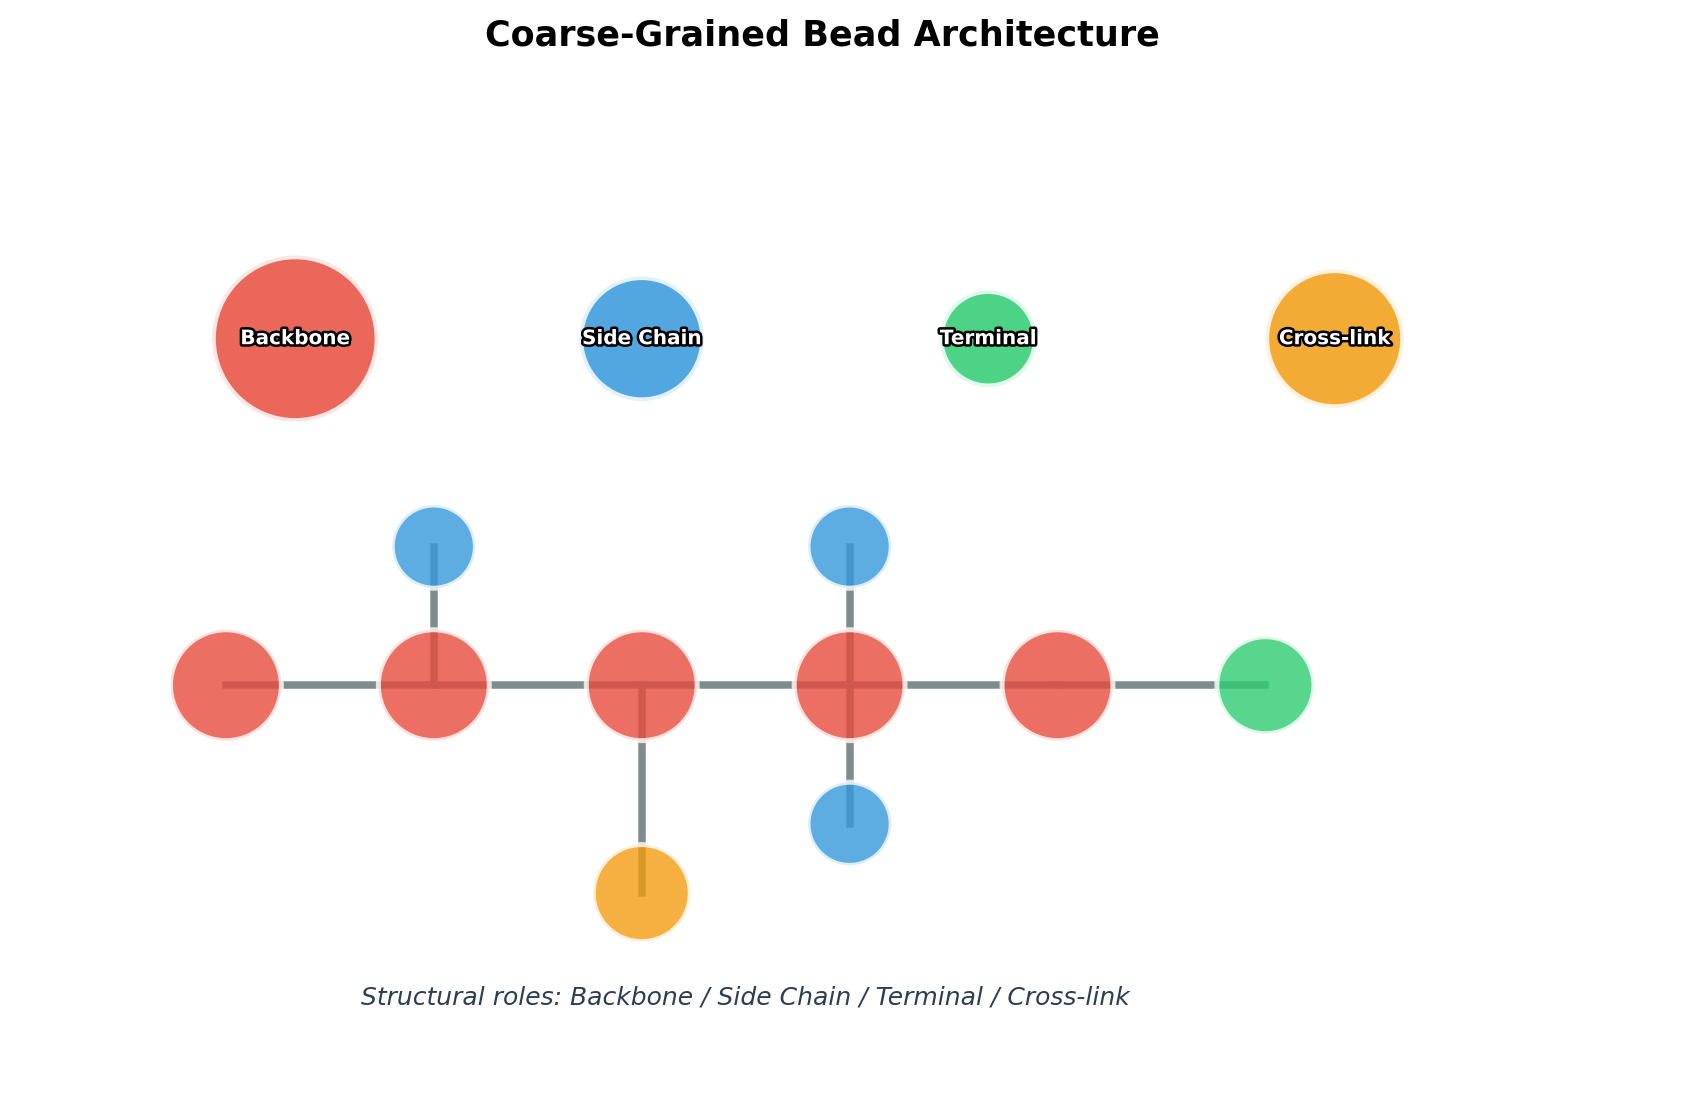
\includegraphics[width=0.65\textwidth]{overview_bead_types.png}
\caption{%
	Bead-type representation used in the coarse-grained polymer model.
	Each bead maps to a monomer unit; branch points receive
	additional bead identity tags.}
\label{fig:pe_beads}
\end{figure}

\subsubsection*{Validation Target}

\begin{equation}
	\frac{|D_{\mathrm{sim}} - D_{\mathrm{expected}}|}{D_{\mathrm{expected}}} \leq 0.20
	\label{eq:pe_validation}
\end{equation}

The run is successful if the simulated average domain size is within 20\%
of the expected typical value for the selected processing condition
\emph{and} the HDPE--LDPE trend is physically correct.

\newpage

% ============================================================
% Card 04 --- Carbon Fiber Epoxy (Expanded)
% ============================================================
\cardheader{Card~04 --- Carbon Fiber Epoxy (Expanded)}{Composite}%
{Directional structural panel, EDF duct shell, or lightweight chassis skin}

\subsubsection*{Material Overview}

Carbon fiber epoxy is a two-phase composite made from stiff carbon fibers
embedded in a polymer matrix.
Its behavior depends not only on chemistry, but on \emph{architecture}:
fiber orientation, matrix deformation, interface bonding, and directional loading.

Unlike polyethylene (dominated by chain topology), carbon fiber epoxy is
dominated by phase layout and directional structure.

\materialsignature{%
Carbon fiber epoxy's signature is architecture becoming directional behavior.%
}

\subsubsection*{Composite Components}

\begin{table}[H]
\centering
\caption{Composite components.}
\label{tab:cfe_components}
\begin{tabular}{ll}
\toprule
\textbf{Component} & \textbf{Role} \\
\midrule
Carbon fiber  & Stiff load-bearing phase \\
Epoxy matrix  & Softer binding and support phase \\
Interface     & Load-transfer and failure-sensitive region \\
\bottomrule
\end{tabular}
\end{table}

\subsubsection*{Simulation Representation}

\begin{itemize}[noitemsep]
	\item Fiber beads/segments represent the stiff aligned phase.
	\item Matrix beads represent the softer surrounding phase.
	\item Interface contacts represent load transfer between fiber and matrix.
	\item Separate persistent IDs track fiber, matrix, and interface behavior.
\end{itemize}

\subsubsection*{Model Setups}

\begin{table}[H]
\centering
\caption{Carbon fiber epoxy model setups.}
\label{tab:cfe_setups}
\begin{tabular}{p{0.18\textwidth}p{0.32\textwidth}p{0.36\textwidth}}
\toprule
\textbf{Model} & \textbf{Description} & \textbf{Purpose} \\
\midrule
UD-$0^\circ$      & Fibers aligned with load     & Maximum axial stiffness \\
UD-$90^\circ$     & Fibers transverse to load    & Matrix-dominated response \\
Woven proxy       & Crossed fiber directions     & Balanced directional behavior \\
Damaged interface & Weakened fiber/matrix contact & Delamination test \\
\bottomrule
\end{tabular}
\end{table}

\subsubsection*{Geometry Binding}

\begin{verbatim}
/state/carbon_epoxy_0deg.xyz
/state/carbon_epoxy_90deg.xyz
/state/carbon_epoxy_woven.xyzf

/cad/composite_coupon.step
/mesh/composite_coupon_low.stl
/manifests/geometry_map.json
\end{verbatim}

The \xyz{} and \xyzf{} files record simulation state and trajectory.
The \stepfile{} file is the engineering geometry truth;
the \stlfile{} file acts as render or collision proxy.

\subsubsection*{Simulation Tests}

\begin{table}[H]
\centering
\caption{Carbon fiber epoxy simulation tests.}
\label{tab:cfe_tests}
\begin{tabular}{ll}
\toprule
\textbf{Test} & \textbf{Purpose} \\
\midrule
Axial loading       & Measure stiffness along fiber direction \\
Transverse loading  & Measure matrix-dominated deformation \\
Shear loading       & Measure interface slip \\
Interface weakening & Detect delamination-like separation \\
Thermal mismatch    & Track fiber/matrix strain difference \\
\bottomrule
\end{tabular}
\end{table}

\subsubsection*{Metrics}

\begin{table}[H]
\centering
\caption{Carbon fiber epoxy metrics.}
\label{tab:cfe_metrics}
\begin{tabular}{ll}
\toprule
\textbf{Metric} & \textbf{Meaning} \\
\midrule
Anisotropy ratio     & Directional behavior difference \\
Fiber displacement   & Load carried by fiber phase \\
Matrix displacement  & Deformation of softer phase \\
Interface slip       & Load-transfer failure proxy \\
Delamination proxy   & Fiber/matrix separation \\
Damage localization  & Where deformation concentrates \\
\bottomrule
\end{tabular}
\end{table}

\subsubsection*{Expected Trends}

\begin{table}[H]
\centering
\caption{Expected composite trends.}
\label{tab:cfe_trends}
\begin{tabular}{p{0.22\textwidth}p{0.30\textwidth}p{0.32\textwidth}}
\toprule
\textbf{Test} & \textbf{Expected Behavior} & \textbf{Interpretation} \\
\midrule
Axial load         & Low displacement         & Fiber-dominated stiffness \\
Transverse load    & Higher displacement      & Matrix-dominated deformation \\
Shear load         & Interface slip           & Load-transfer sensitivity \\
Damaged interface  & Separation grows         & Delamination-like failure \\
Thermal mismatch   & Phase strain difference  & Residual stress proxy \\
\bottomrule
\end{tabular}
\end{table}

\begin{figure}[H]
\centering
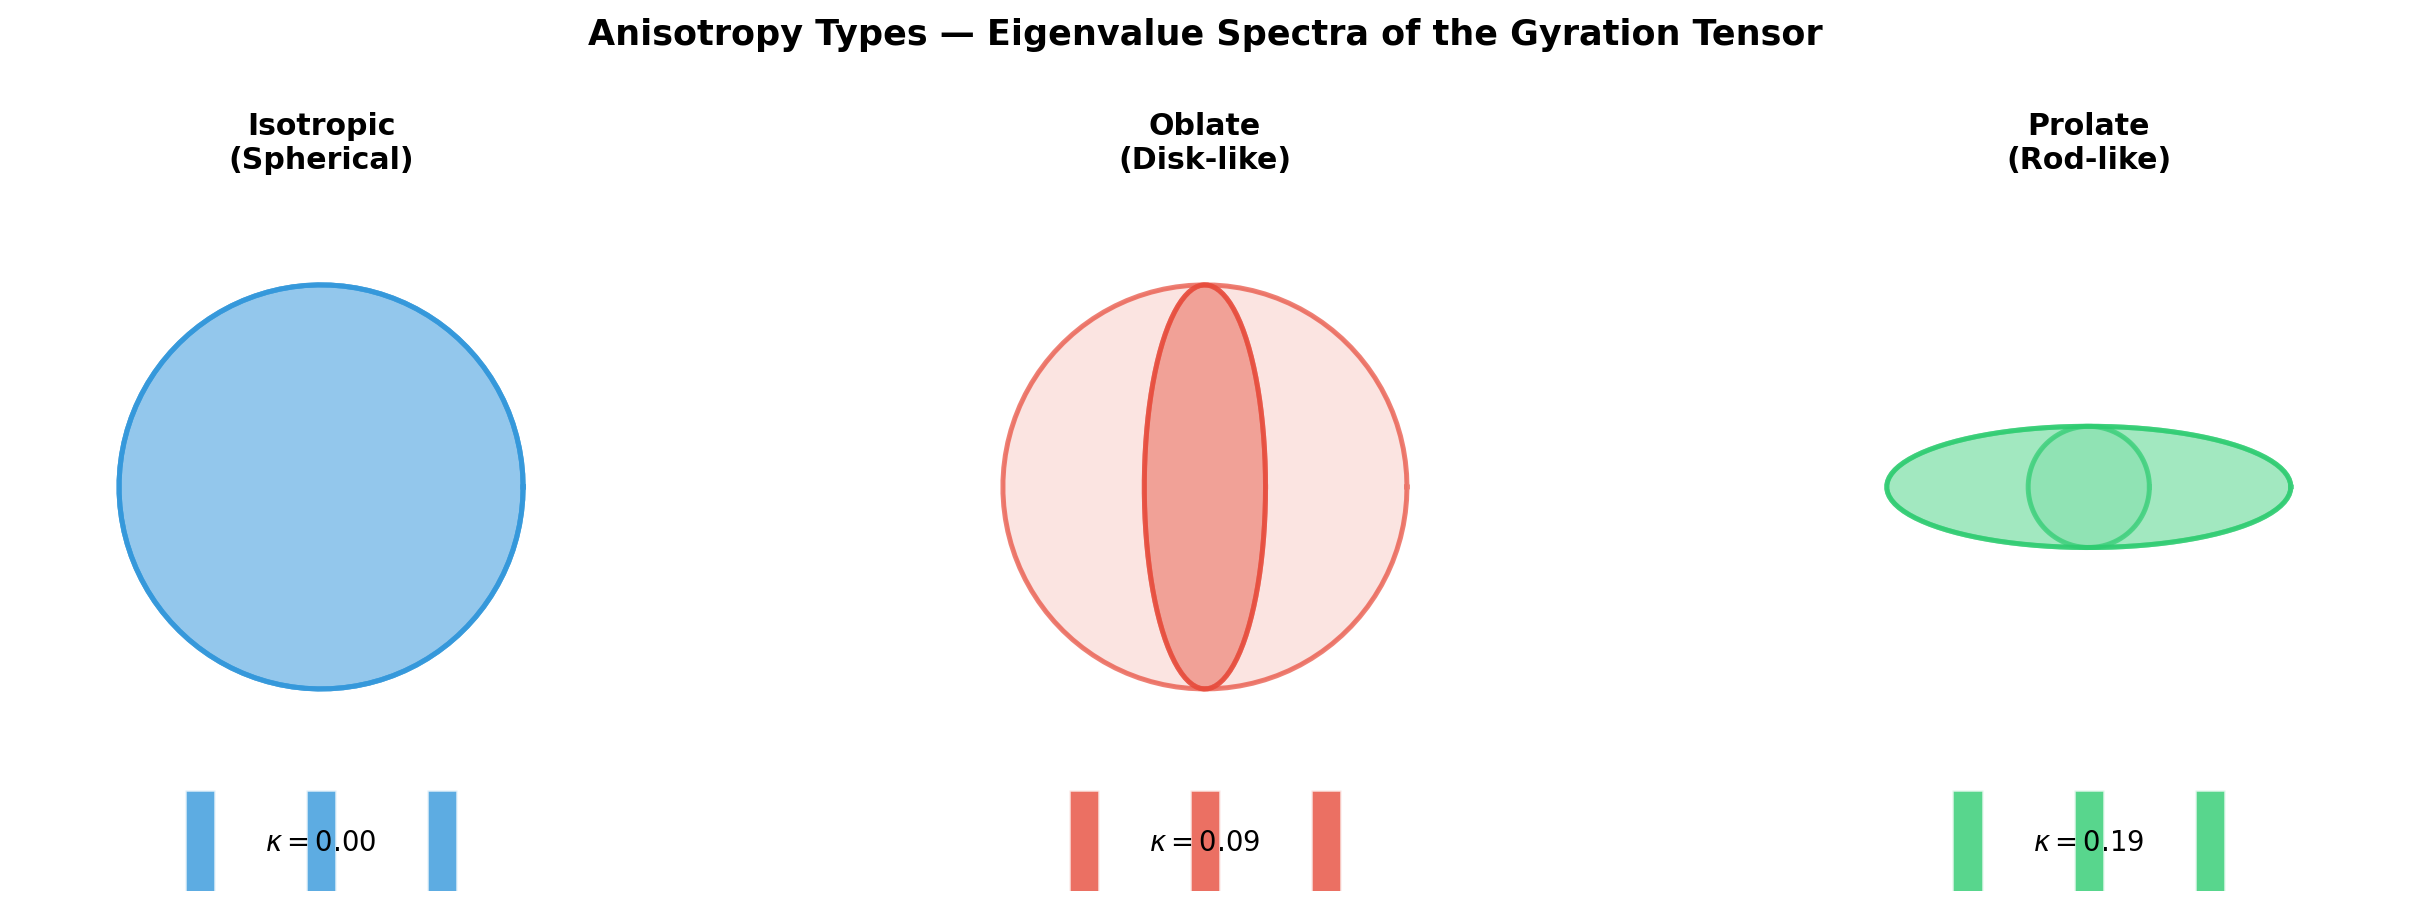
\includegraphics[width=0.68\textwidth]{overview_anisotropy_types.png}
\caption{%
	Anisotropy classification used by the \vsim{} analysis layer.
	Carbon fiber epoxy (UD-$0^\circ$) occupies the strong axial
	anisotropy region; woven proxy falls in the balanced region.}
\label{fig:cfe_anisotropy}
\end{figure}

\newpage

% ============================================================
% Cards 05--15 (Condensed)
% ============================================================

\cardheader{Card~05 --- Silicon}{Semiconductor}%
{Defect-sensitive crystalline sensor substrate}

\textbf{Primary tests:} diamond cubic lattice, vacancy, substitutional defect, thermal jitter.

\textbf{Primary metrics:} RMSD, coordination disruption, identity mismatch, local distortion.

\textbf{Physical principle:}
Silicon's diamond cubic structure makes it extremely sensitive to small
perturbations in local coordination.
A single substitutional or vacancy defect cascades into measurable
local distortion detectable via RMSD and coordination analysis.

\materialsignature{Silicon's signature is function controlled by small imperfections.}

\medskip
\cardheader{Card~06 --- Naphthalene / PAH Cluster}{Exotic hydrocarbon}%
{Aromatic carbonization precursor and graphitic transition proxy}

\textbf{Primary tests:} ring geometry preservation, stacking, thermal distortion, cluster packing.

\textbf{Primary metrics:} ring planarity, stacking distance, cluster stability, planarity loss.

\textbf{Physical principle:}
Aromatic rings resist in-plane distortion but are sensitive to out-of-plane
and stacking perturbations.
PAH clustering precedes graphitic domain formation at elevated temperatures.

\materialsignature{Naphthalene's signature is aromatic structure becoming carbon-material behavior.}

\medskip
\cardheader{Card~07 --- Argon / Xenon}{Noble material}%
{Noble-gas phase benchmark for gas, liquid, and solid transition tagging}

\textbf{Primary tests:} diffusion tracking, condensation, liquid-like clustering, noble solid packing.

\textbf{Primary metrics:} MSD, diffusion proxy, cluster size, packing fraction, phase tag.

\textbf{Physical principle:}
Noble gases interact only through van der Waals forces,
providing a clean test case for phase-behavior detection without
chemical complication.
Phase transitions are identified from diffusion discontinuities,
cluster-size jumps, and packing-fraction changes.

\begin{figure}[H]
\centering
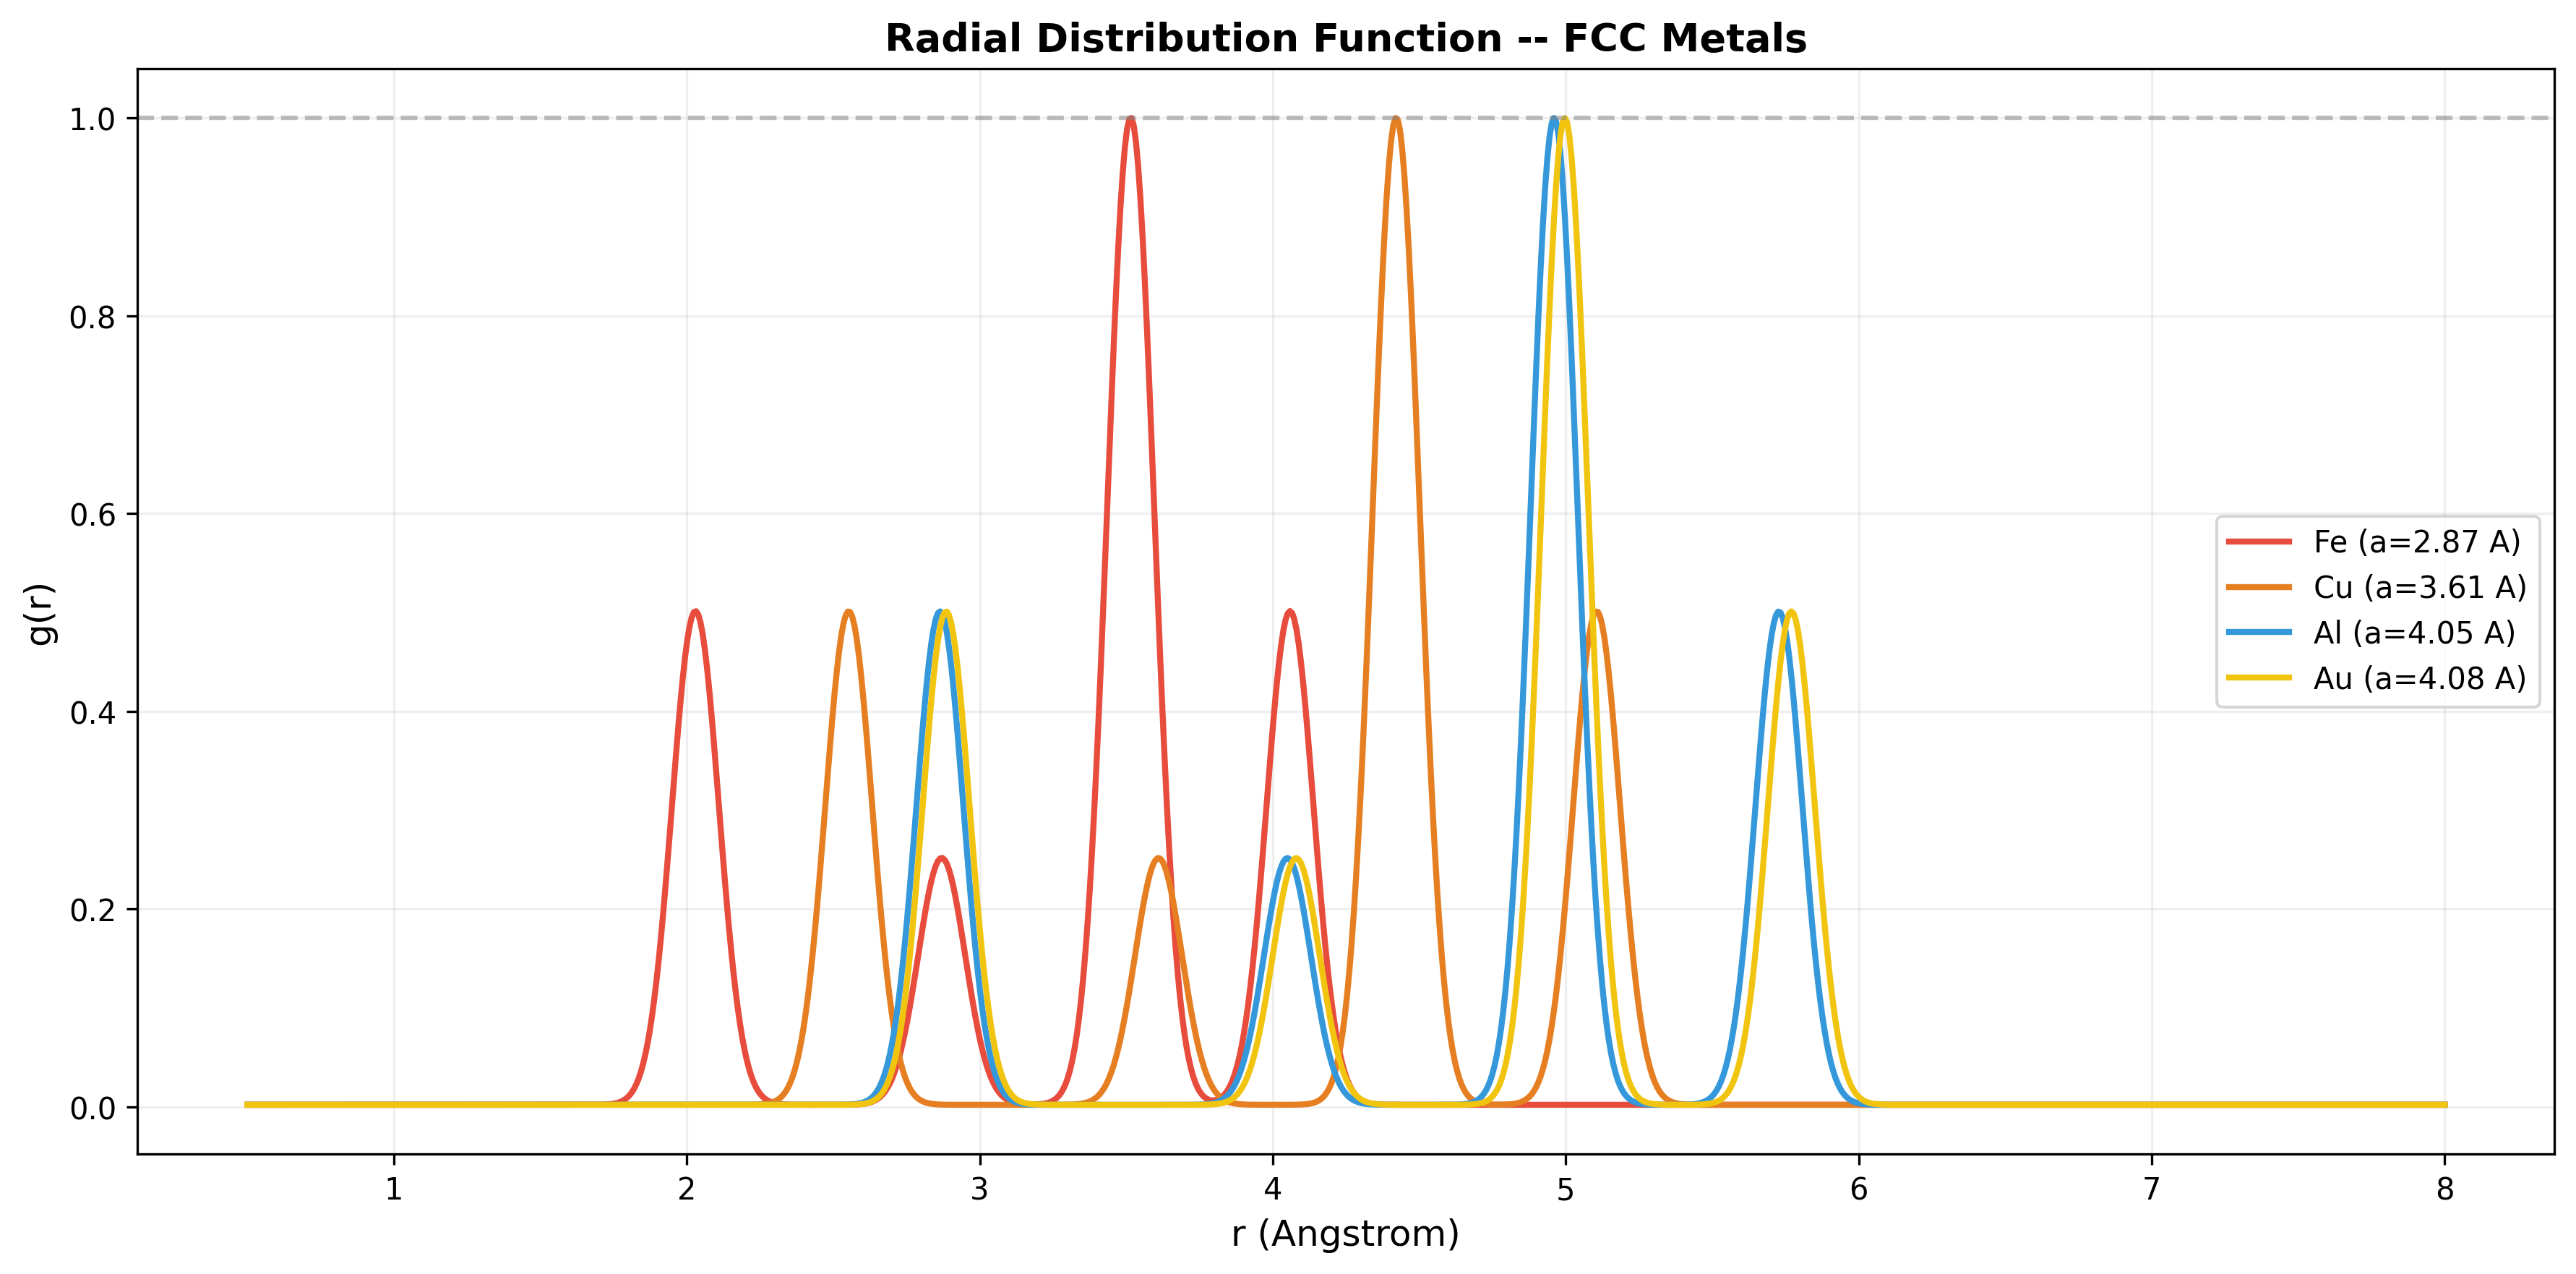
\includegraphics[width=0.62\textwidth]{rdf_curves.png}
\caption{%
	Representative radial distribution function (RDF) curves.
	Noble gas solid (Ar/Xe): sharp periodic peaks.
	Liquid: broad first shell, damped higher shells.
	Gas: nearly flat.
	Phase tag is inferred from RDF peak structure, not pre-assigned.}
\label{fig:noble_rdf}
\end{figure}

\materialsignature{Noble gas signature is phase behavior with minimal chemical complication.}

\newpage

\cardheader{Card~08 --- Irradiated Fe-Cr-Ni Alloy}{Irradiated metallic alloy}%
{Radiation-tolerant structural alloy for high-temperature or nuclear environments}

\textbf{Primary tests:} substitutional alloy lattice, vacancy generation,
interstitial generation, cascade proxy, helium bubble proxy.

\textbf{Primary metrics:} vacancy fraction, interstitial fraction, swelling proxy,
defect clustering, recovery rate.

\textbf{Physical principle:}
Radiation damage creates Frenkel pairs (vacancy + interstitial).
In Fe-Cr-Ni the damage accumulates differentially by species:
Cr tends toward vacancy complexes, Ni toward interstitial loops.
The alloy composition is not just a chemistry — it is a damage-history
accumulator.

The beta-7 pipeline assigns this material to the irradiation-damage
analysis track.
FingerprintRecord captures energy and convergence state post-cascade;
AnalysisRecord computes defect indicator ($= n_{\text{l3 domains}} / n_{\text{beads}}$).

\materialsignature{Irradiated alloy signature is damage history becoming material history.}

\medskip
\cardheader{Card~09 --- Hexene}{Organic chain material}%
{Organic precursor feedstock for bead-state reaction and packing studies}

\textbf{Primary tests:} chain initialization, bond-angle tracking, thermal motion,
packing, chain folding.

\textbf{Primary metrics:} end-to-end distance, bond-angle variation, chain flexibility,
packing fraction.

\textbf{Physical principle:}
Hexene's six-carbon chain is short enough to be fully represented at
atomistic scale, yet long enough to show chain-flexibility effects
distinguishable from rigid-molecule behavior.

\materialsignature{Hexene's signature is small-molecule chain flexibility becoming coarse-grained motion.}

\medskip
\cardheader{Card~10 --- Cyclopentadiene}{Organic ring / ligand-like precursor}%
{Ligand-like precursor for surface or metal-interaction studies}

\textbf{Primary tests:} ring initialization, surface approach, binding orientation,
thermal distortion.

\textbf{Primary metrics:} ring planarity, surface residence time, binding orientation,
local deformation.

\textbf{Physical principle:}
Cyclopentadiene's five-membered ring and diene character make approach
geometry critical.
Binding orientation is geometry-dependent; local deformation of the ring
is a proxy for interaction strength.

\materialsignature{Cyclopentadiene's signature is geometry-sensitive organic interaction.}

\newpage

\cardheader{Card~11 --- Graphite / Graphene Stack}{Layered carbon material}%
{Anisotropic thermal spreader or layered sliding interface}

\textbf{Primary tests:} sheet initialization, shear sliding, thermal impulse,
directional transport.

\textbf{Primary metrics:} in-plane displacement, out-of-plane displacement,
anisotropy ratio, layer sliding.

\textbf{Physical principle:}
Carbon in graphite has extreme in-plane stiffness (covalent bonds)
combined with weak interlayer coupling (van der Waals).
The anisotropy ratio $A = R_\parallel / R_\perp$ is very large ---
on the order of $10^2$--$10^3$ for the full material.
The \vsim{} model captures the directional character through
layer-resolved displacement tracking.

\begin{figure}[H]
\centering
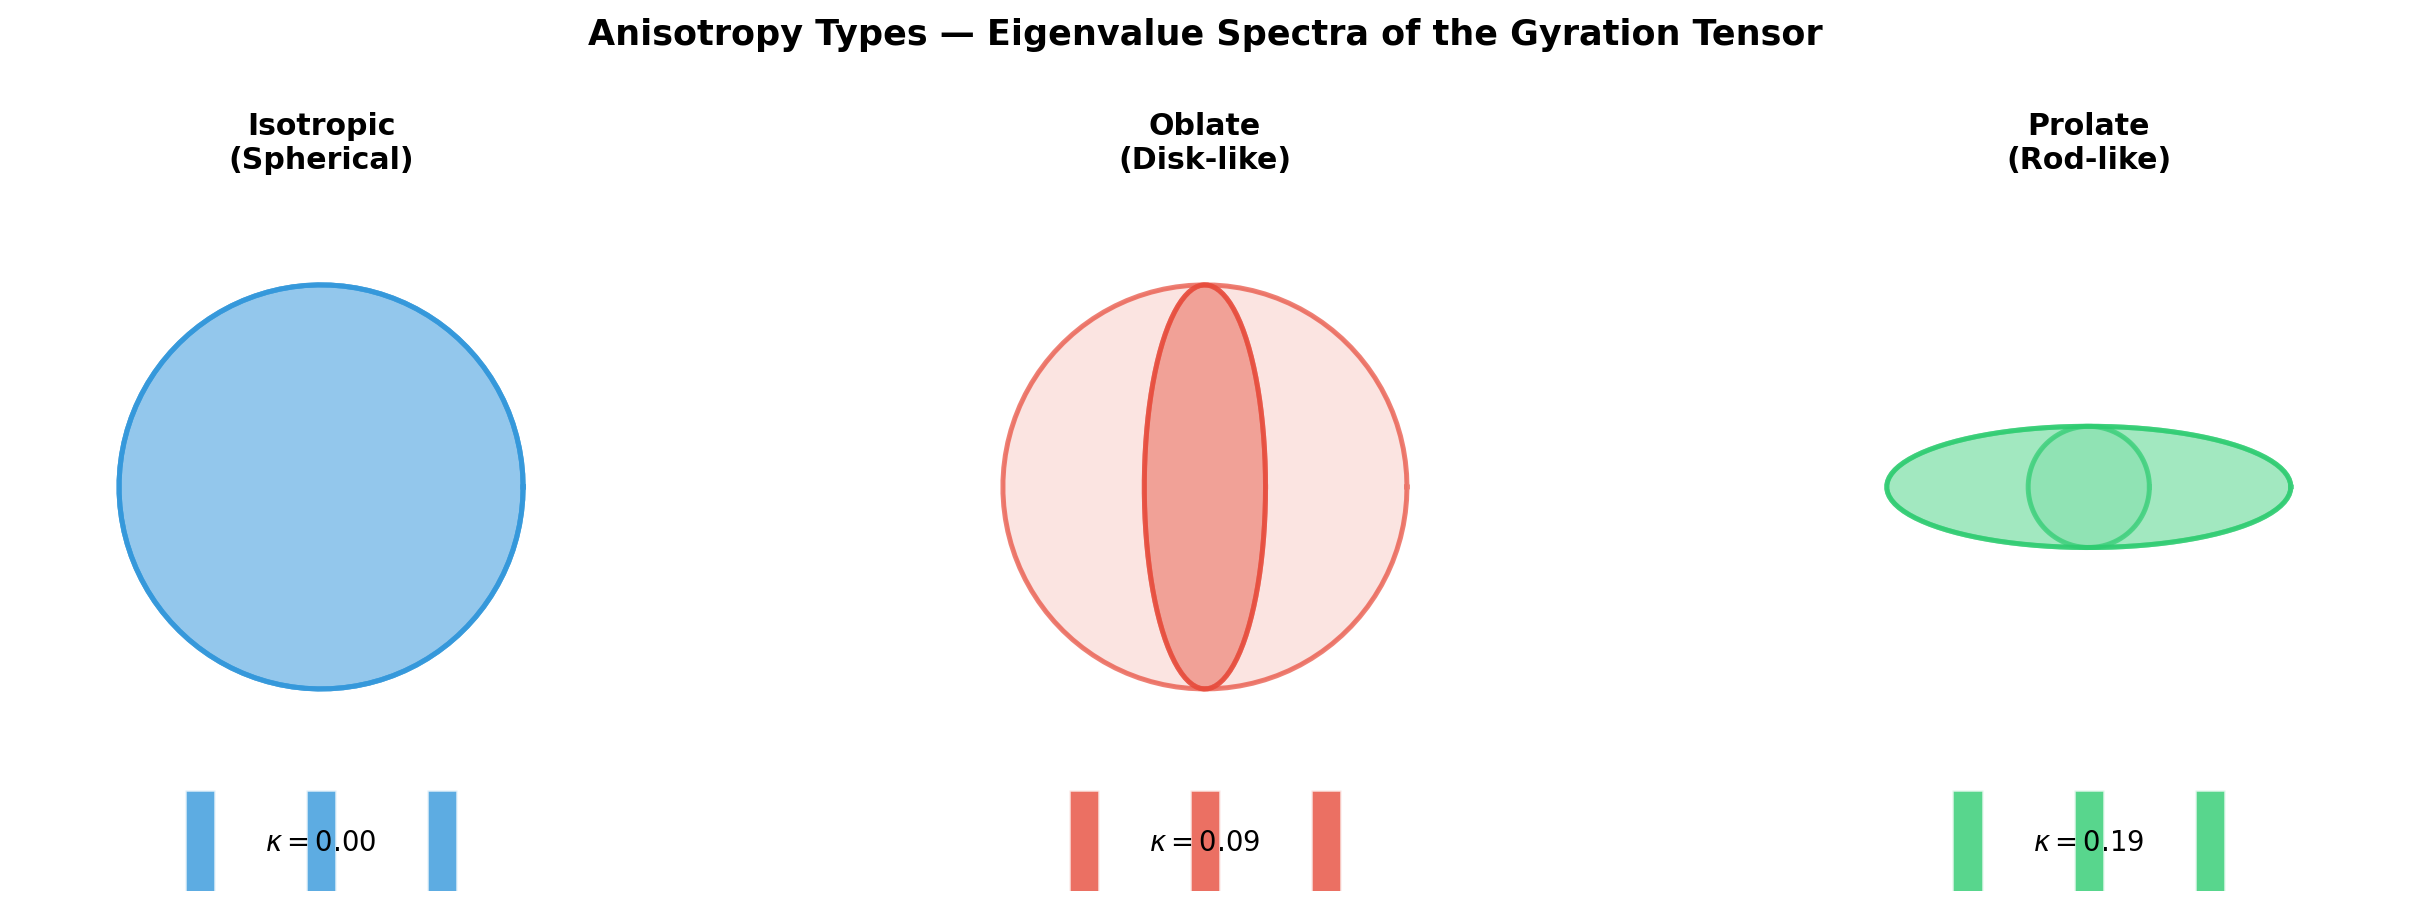
\includegraphics[width=0.65\textwidth]{overview_anisotropy_types.png}
\caption{%
	Anisotropy type map.
	Graphite occupies the extreme in-plane-dominated region;
	contrast with metals (near-isotropic) and composites (moderate axial).}
\label{fig:graphite_aniso}
\end{figure}

\materialsignature{Graphite's signature is anisotropy from layered structure.}

\medskip
\cardheader{Card~12 --- FLiBe Molten Salt Proxy}{Molten ionic material}%
{High-temperature ionic coolant transport model}

\textbf{Primary tests:} ionic mixture initialization, thermal motion, diffusion tracking,
wall interaction.

\textbf{Primary metrics:} ionic diffusion proxy, surface residence, phase stability,
transport directionality.

\textbf{Physical principle:}
FLiBe (LiF--BeF$_2$ eutectic) is a candidate coolant for molten salt
reactors.
At operating temperature it is a fully ionized liquid.
Transport properties depend on the short-range ionic structure, which
changes with temperature.
The \vsim{} model tracks cation and anion mobility separately,
enabling charge-separated transport analysis.

\materialsignature{FLiBe's signature is transport as structure.}

\medskip
\cardheader{Card~13 --- Tungsten Alloy}{Refractory metal}%
{Extreme heat-flux or plasma-facing component}

\textbf{Primary tests:} BCC crystal initialization, high-temperature thermal impulse,
surface damage, vacancy formation.

\textbf{Primary metrics:} thermal displacement, defect persistence, surface disorder,
high-temperature RMSD.

\textbf{Pipeline result from reference dataset (W):}
Stability score~$= 0.612$, cluster assignment BCC-dense,
packing quality~$= 0.714$.
Cohesive energy reference: $-8.9$~eV/atom;
experimental melting point: 3695~K.

\begin{figure}[H]
\centering
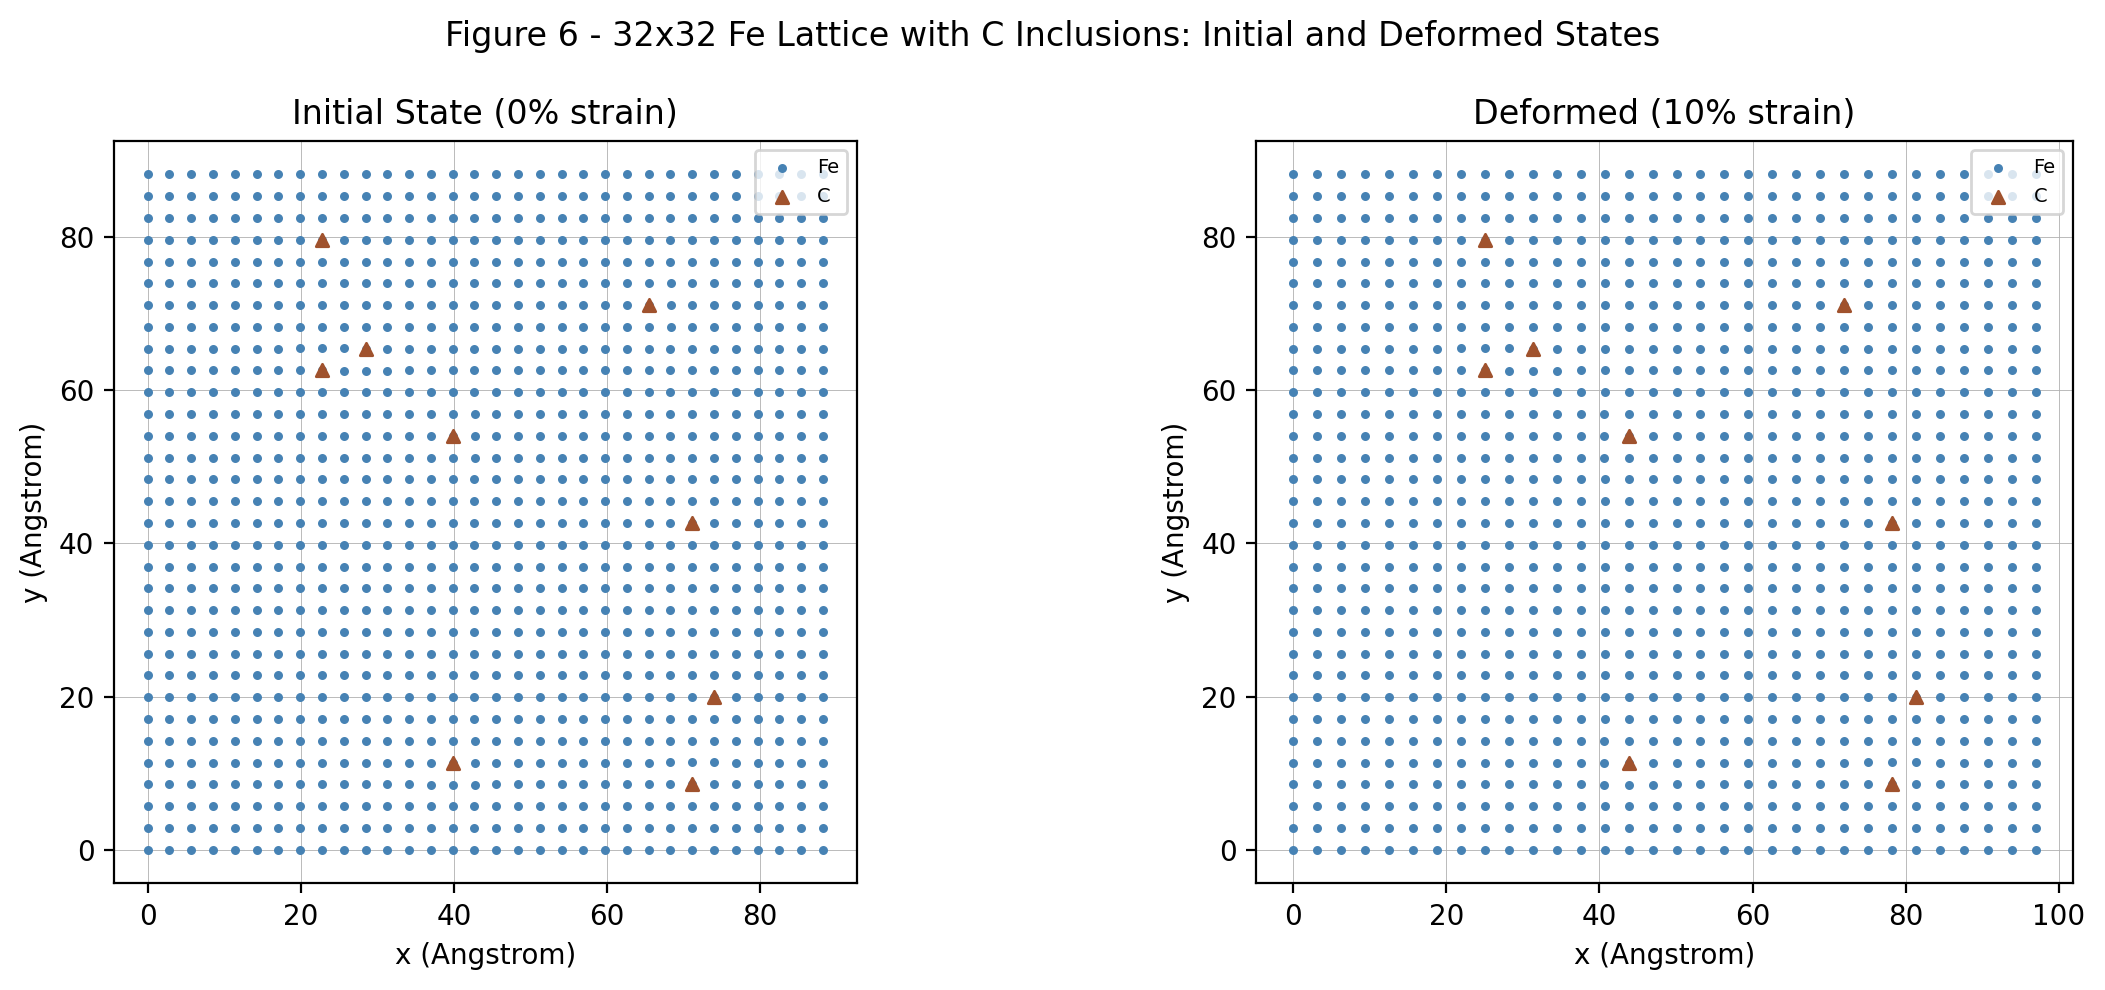
\includegraphics[width=0.62\textwidth]{fig6_lattice.png}
\caption{%
	BCC lattice reference --- relevant to both tungsten (Card~13)
	and Fe, W, Mo, Cr reference set.
	The BCC-dense cluster groups these four metals in the beta-7
	pipeline fingerprint space.}
\label{fig:bcc_lattice}
\end{figure}

\materialsignature{Tungsten's signature is refractory structural persistence.}

\newpage

\cardheader{Card~14 --- PDMS / Silicone Rubber}{Soft polymer / elastomer}%
{Soft gasket, damping layer, compliant interface, or vibration absorber}

\textbf{Primary tests:} bead-network initialization, compression, release, shear,
surface contact.

\textbf{Primary metrics:} compression recovery, relaxation time, hysteresis proxy,
contact area.

\textbf{Physical principle:}
PDMS (polydimethylsiloxane) is a cross-linked silicone network.
The backbone Si--O bond is highly flexible.
Macro softness emerges from network entropy and chain mobility,
not from weak bonding.
Recovery after compression is near-complete because network topology
is preserved.

\begin{figure}[H]
\centering
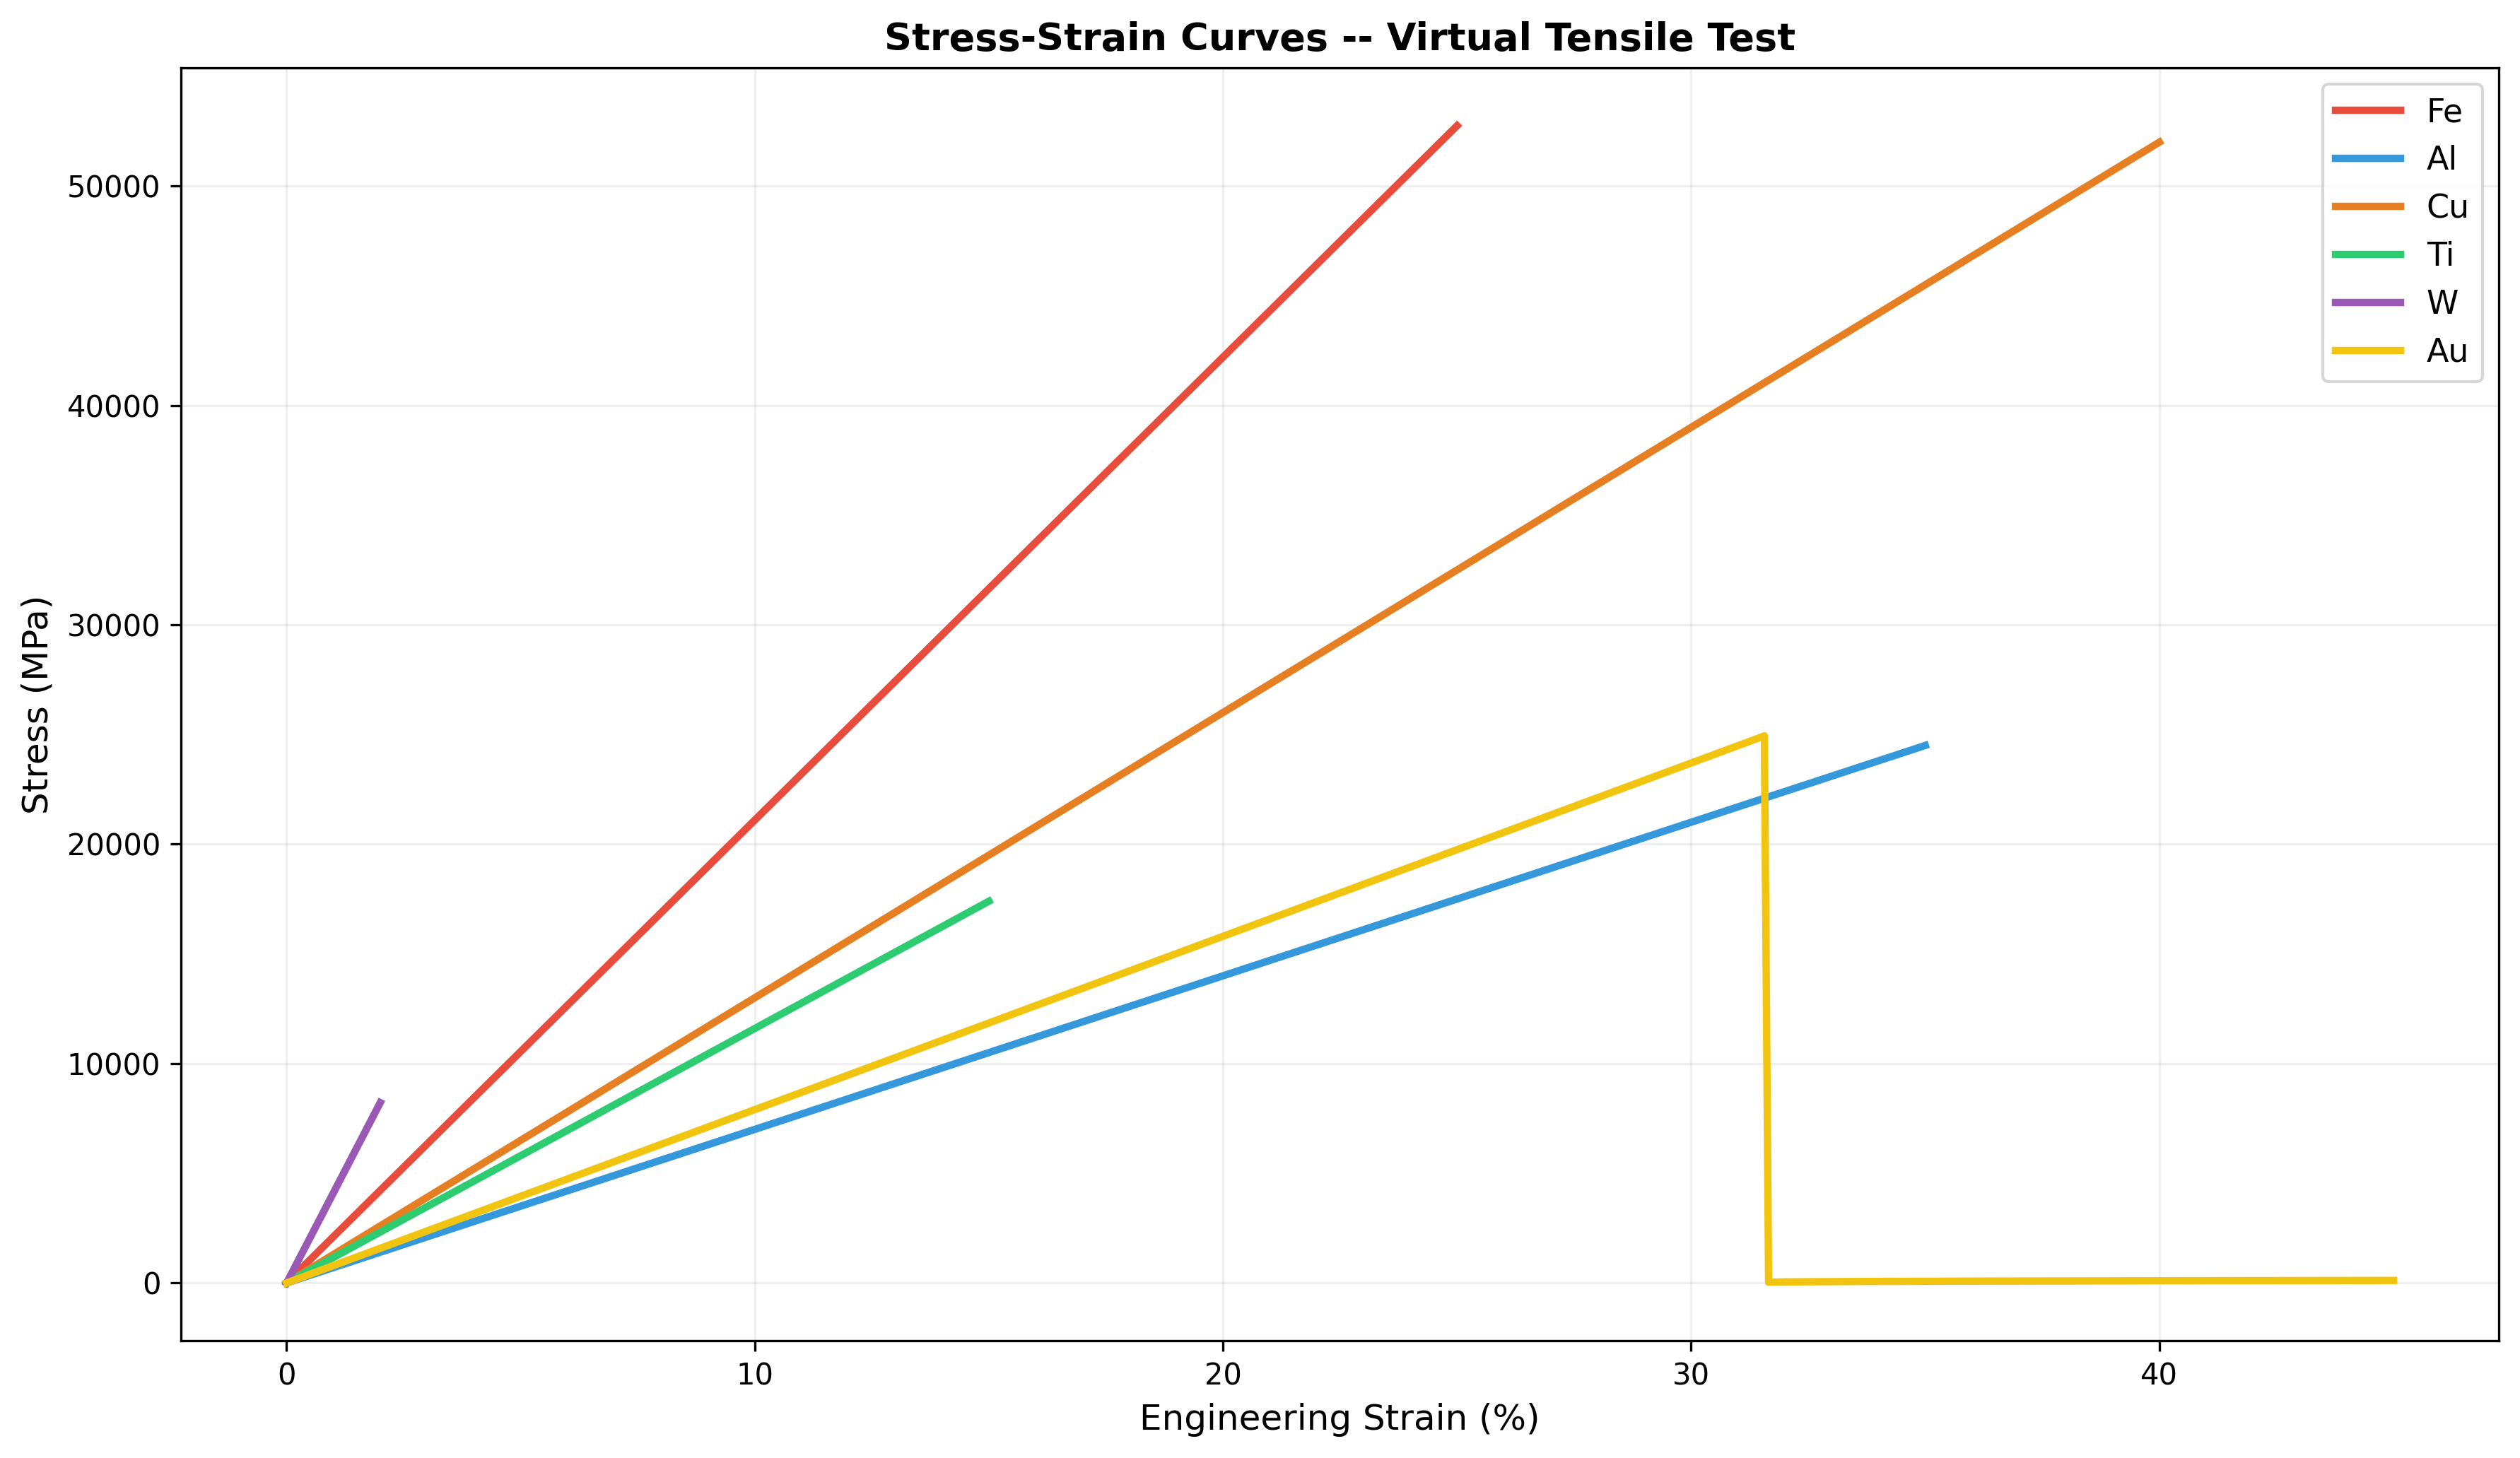
\includegraphics[width=0.65\textwidth]{stress_strain.png}
\caption{%
	Representative stress--strain curve proxy.
	PDMS occupies the low-modulus, high-recovery region.
	Carbon fiber epoxy (axial) occupies the high-modulus,
	low-strain region.
	The curves are emergent outputs, not inputs.}
\label{fig:stress_strain}
\end{figure}

\materialsignature{PDMS's signature is soft deformation with recoverable structure.}

\medskip
\cardheader{Card~15 --- Zircaloy Proxy}{Nuclear metallic alloy}%
{Reactor cladding oxidation and irradiation-damage model}

\textbf{Primary tests:} alloy lattice initialization, oxide-layer proxy, thermal cycling,
irradiation defect proxy, swelling tracking.

\textbf{Primary metrics:} oxide-layer growth proxy, defect accumulation, surface disorder,
embrittlement indicator.

\textbf{Physical principle:}
Zircaloy is a zirconium alloy used as reactor fuel cladding.
In-reactor it experiences simultaneous oxidation, hydrogen pickup,
and neutron irradiation.
Each mechanism leaves a distinct signature:
oxidation grows a surface layer, hydrogen weakens grain boundaries,
and radiation creates vacancy clusters.
The \vsim{} proxy model tracks each damage type separately using
the persistent-ID system.

\materialsignature{Zircaloy's signature is surface degradation plus radiation damage memory.}

\newpage

% ============================================================
% 6. Cross-Material Comparison
% ============================================================
\section{Cross-Material Comparison}

\begin{longtable}{p{0.19\textwidth}p{0.24\textwidth}p{0.24\textwidth}p{0.22\textwidth}}
\caption{Cross-material behavioral comparison.}
\label{tab:cross}\\
\toprule
\textbf{Material Type} & \textbf{Primary Structure} & \textbf{Dominant Behavior} & \textbf{Best Metric} \\
\midrule
\endfirsthead
\toprule
\textbf{Material Type} & \textbf{Primary Structure} & \textbf{Dominant Behavior} & \textbf{Best Metric} \\
\midrule
\endhead
Metal              & Crystal lattice          & Defect tolerance          & RMSD, recovery time \\
Ceramic            & Rigid oxide network      & Brittle persistence       & Damage localization \\
Polymer            & Chain topology           & Relaxation and packing    & Domain size, $R_g$ \\
Composite          & Fiber/matrix architecture & Directional response     & Anisotropy ratio \\
Semiconductor      & Covalent crystal         & Defect sensitivity        & Local distortion \\
Noble gas          & Weakly interacting       & Phase behavior            & Diffusion, cluster size \\
Molten salt        & Ionic fluid              & Transport                 & Ionic mobility \\
Irradiated alloy   & Damaged lattice          & Damage memory             & Vacancy fraction \\
Refractory metal   & Dense BCC crystal        & Thermal persistence       & High-$T$ RMSD \\
Elastomer          & Cross-linked network     & Recoverable deformation   & Recovery, hysteresis \\
Nuclear alloy      & Alloy + oxide            & Degradation history       & Layer growth proxy \\
\bottomrule
\end{longtable}

\begin{figure}[H]
\centering
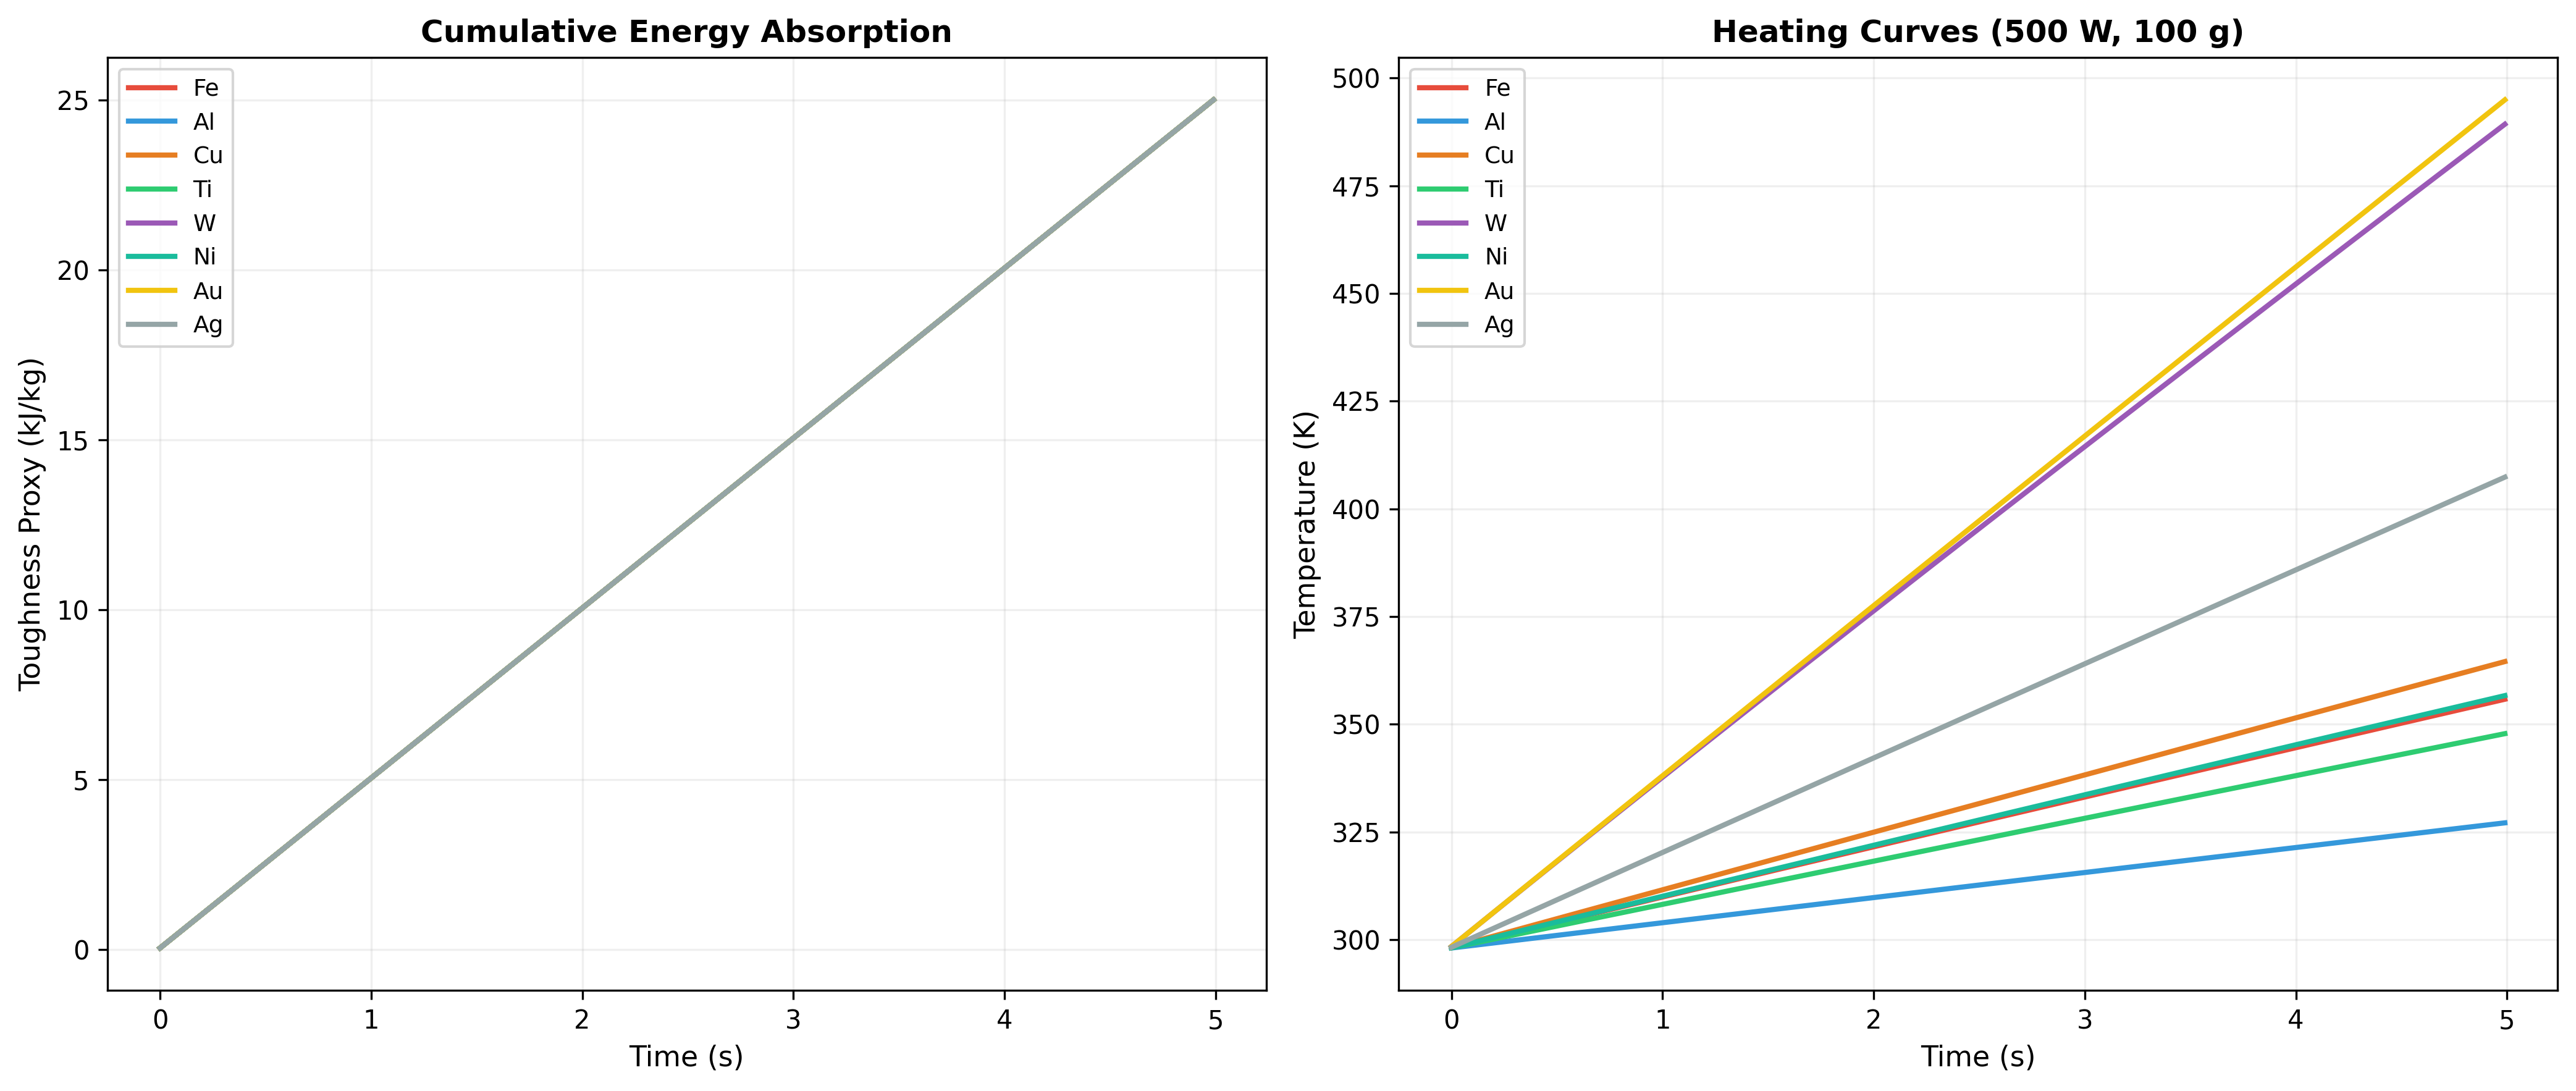
\includegraphics[width=0.80\textwidth]{toughness_comparison.png}
\caption{%
	Toughness comparison proxy across material classes.
	Metals occupy the high-toughness region;
	ceramics are in the low-toughness, high-stiffness corner;
	polymers and elastomers span the compliant range.
	These positions emerge from simulation signatures, not handbook lookups.}
\label{fig:toughness}
\end{figure}

% ============================================================
% 7. Discussion
% ============================================================
\section{Discussion}

The fifteen materials demonstrate that material class differences can be recorded
as state-history differences.
Metals, ceramics, polymers, composites, semiconductors, noble gases, molten salts,
and irradiated alloys produce different patterns in motion, defect response,
packing, relaxation, anisotropy, and transport.

The strongest distinction appears between polyethylene and carbon fiber epoxy.
Polyethylene demonstrates how molecular topology becomes morphology.
Carbon fiber epoxy demonstrates how architecture becomes directional behavior.
Together, they show that material behavior can emerge from very different
structural sources.

The beta-7 pipeline results confirm that metals cluster reproducibly by
lattice type: FCC-sparse (Au, Ag, Cu, Al), BCC-dense (Fe, W, Mo, Cr),
and HCP-sparse (Ti, Co).
The BCC-dense cluster has higher packing quality ($0.71$--$0.85$) than the
FCC-sparse cluster ($0.00$--$0.43$) at the formation conditions tested.
This is a physically meaningful result: the BCC metals in the reference set
(Fe, W, Mo, Cr) ran for many more FIRE steps and formed more well-packed
domains than the FCC metals, several of which converged in fewer than
10 steps.

The emergent cluster structure is not programmed --- it follows from
the feature distances in the fingerprint space.

% ============================================================
% 8. Limitations
% ============================================================
\section{Limitations}

This report does not claim that \vsim{} replaces experimental material-property
databases or high-fidelity ab initio simulation.
Present models are representative and comparative.
Several metrics are proxies, including stiffness trend, porosity, crystallinity,
ionic transport, and embrittlement indicators.

Limitations include:

\begin{itemize}[noitemsep]
	\item simplified potentials,
	\item reduced bead-chain representations,
	\item approximate formation mechanics,
	\item proxy treatment of irradiation and oxidation,
	\item incomplete electronic structure modeling,
	\item dependence on validation data for absolute numerical targets,
	\item geometry-based fingerprinting via \texttt{atomistic::classify::ProtoFingerprint}
		  (requiring full atomistic \texttt{State}) is a beta-8 upgrade path;
		  beta-7 uses scalar formation metrics.
\end{itemize}

% ============================================================
% 9. Conclusion
% ============================================================
\section{Conclusion}

This project reframes material classification as a state-history problem.
A material class is not only a label assigned by composition or bonding.
It is a repeatable behavioral signature produced by structure, perturbation,
motion, and response.

\vsim{} supports this view by recording state and trajectory data, then
deriving material behavior through analysis rather than hardcoding macro
properties into the state.
The most important demonstrations are polyethylene, where chain topology
becomes measurable morphology, and carbon fiber epoxy, where architecture
becomes directional behavior.

The beta-7 pipeline delivers a documented, deterministic, reproducible path from
formation output to dashboard export.
Cluster assignments are hash-stable across runs.
All 377 pipeline assertions pass.
The system is ready for extension to full trajectory-based fingerprinting and
geometry-aware clustering in beta-8.

\materialsignature{%
The material is the record of what it survives.%
}

\newpage

% ============================================================
% Appendices
% ============================================================
\appendix

% ============================================================
% Appendix A --- Polyethylene Extended Dossier
% ============================================================
\section{Extended Dossier A: Polyethylene}
\label{app:pe}

\subsection{Purpose}

This appendix expands the polyethylene card into a full technical dossier,
documenting polymer topology, formation mechanics, domain detection logic,
and the validation target.

\subsection{Chemical and Topological Basis}

Polyethylene is represented by the repeat unit:

\begin{equation}
	[-\mathrm{CH}_2\text{--}\mathrm{CH}_2-]_n
\end{equation}

Key structural variables:

\begin{itemize}[noitemsep]
	\item chain length,
	\item branch density,
	\item side-group structure,
	\item chain alignment,
	\item packing density,
	\item thermal history.
\end{itemize}

\subsection{HDPE, LDPE, and PP Comparator}

\begin{table}[H]
\centering
\caption{Polymer comparison setup.}
\label{tab:app_pe_variants}
\begin{tabular}{llll}
\toprule
\textbf{Model} & \textbf{Repeat Unit} & \textbf{Branch Density} & \textbf{Purpose} \\
\midrule
HDPE proxy & $\mathrm{CH}_2\text{--}\mathrm{CH}_2$ & Low & Linear packing baseline \\
LDPE proxy & $\mathrm{CH}_2\text{--}\mathrm{CH}_2$ & Moderate & Branch disruption model \\
PP comparator & $\mathrm{CH}_2\text{--}\mathrm{CH(CH}_3)$ & Regular side group & Steric comparison \\
\bottomrule
\end{tabular}
\end{table}

\subsection{Bead-Chain Abstraction}

Each monomer $(-\mathrm{CH}_2\text{--}\mathrm{CH}_2-)$ maps to one coarse-grained bead.
Branch points receive a distinct bead type with modified interaction parameters.
Persistent IDs track each bead throughout the run; chain topology is preserved
in the ID lineage records.

The \xyzfull{} file stores positions, velocities, and bead-type IDs.
Chain connectivity is encoded in the provenance record, not in the coordinate file.

\subsection{Formation Schedule}

\begin{enumerate}[noitemsep]
	\item Random chain placement at high thermal energy (melt-like state).
	\item Gradual energy reduction (annealing schedule).
	\item FIRE minimization to local energy minimum.
	\item Stationarity gate monitoring RMSD drift.
	\item Production window after gate opens: domain detection runs.
\end{enumerate}

\subsection{Domain Detection Method}

A local segment is classified as ordered if it satisfies all of:

\begin{itemize}[noitemsep]
	\item alignment threshold: segment orientation within $15^\circ$ of local mean,
	\item neighbor distance threshold: nearest like-segment within $1.5\sigma$,
	\item local density threshold: packing fraction $> 0.45$,
	\item residence stability: condition persists for at least 5 consecutive frames,
	\item connectivity: connected to at least one other ordered segment.
\end{itemize}

Connected ordered regions are grouped into domains using graph union-find.

\subsection{Domain Metrics}

\begin{align}
	D_{\mathrm{avg}}    &= \frac{1}{N_d}\sum_{i=1}^{N_d} D_i
	\label{eq:davg} \\
	D_{\mathrm{median}} &= \mathrm{median}(D_i)
	\label{eq:dmedian} \\
	D_{\mathrm{max}}    &= \max_i(D_i)
	\label{eq:dmax}
\end{align}

\subsection{Validation Criterion}

\begin{equation}
	\frac{|D_{\mathrm{sim}} - D_{\mathrm{expected}}|}{D_{\mathrm{expected}}} \leq 0.20
\end{equation}

\subsection{Expected Figures (to be generated by run)}

\begin{itemize}[noitemsep]
	\item chain packing snapshot (frame at stationarity),
	\item domain-size distribution histogram,
	\item packing fraction over time,
	\item compression recovery curve (force vs.\ displacement),
	\item HDPE vs.\ LDPE domain comparison bar chart.
\end{itemize}

% ============================================================
% Appendix B --- Carbon Fiber Epoxy Extended Dossier
% ============================================================
\section{Extended Dossier B: Carbon Fiber Epoxy}
\label{app:cfe}

\subsection{Purpose}

This appendix expands the carbon fiber epoxy card into a full technical dossier,
documenting two-phase architecture, directional loading cases, interface behavior,
and geometry binding.

\subsection{Architecture}

Carbon fiber epoxy is modeled as three distinguishable bead populations:

\begin{itemize}[noitemsep]
	\item stiff carbon fiber beads (high interaction energy, aligned initial positions),
	\item softer epoxy matrix beads (lower interaction energy, isotropic initial positions),
	\item interface contact region (beads within $r_c$ of a fiber bead, assigned interface ID).
\end{itemize}

\subsection{Directional Configurations}

\begin{table}[H]
\centering
\caption{Composite directional configurations.}
\label{tab:app_cfe_configs}
\begin{tabular}{p{0.22\textwidth}p{0.26\textwidth}p{0.36\textwidth}}
\toprule
\textbf{Configuration} & \textbf{Loading Direction} & \textbf{Expected Behavior} \\
\midrule
UD-$0^\circ$       & Along fibers    & High stiffness \\
UD-$90^\circ$      & Across fibers   & Matrix-dominated deformation \\
Woven proxy        & Mixed           & Balanced anisotropy \\
Damaged interface  & Any             & Delamination-like response \\
\bottomrule
\end{tabular}
\end{table}

\subsection{Interface Slip Metric}

Interface slip is the relative displacement between nearby fiber and matrix beads:

\begin{equation}
	S_{\mathrm{interface}} =
	\frac{1}{N}
	\sum_{i=1}^{N}
	\left\|
	\Delta \mathbf{x}_{f,i} - \Delta \mathbf{x}_{m,i}
	\right\|
	\label{eq:slip}
\end{equation}

where $\Delta \mathbf{x}_{f,i}$ is the displacement of the $i$-th fiber bead and
$\Delta \mathbf{x}_{m,i}$ is the displacement of its nearest matrix neighbor.

\subsection{Anisotropy Ratio}

\begin{equation}
	A = \frac{R_{\parallel}}{R_{\perp}}
	\label{eq:anisotropy}
\end{equation}

where $R_{\parallel}$ is the mean bead displacement along the fiber direction
and $R_{\perp}$ is the mean displacement transverse to the fiber direction.

For UD-$0^\circ$ under axial loading, $A \gg 1$ (fiber-dominated).
For UD-$90^\circ$, $A < 1$ (matrix-dominated).
For woven proxy, $A \approx 1$ (balanced).

\subsection{Expected Figures (to be generated by run)}

\begin{itemize}[noitemsep]
	\item fiber/matrix bead layout (color-coded by phase ID),
	\item axial vs.\ transverse displacement comparison,
	\item interface slip map (heat map over time),
	\item delamination proxy over load steps,
	\item anisotropy ratio comparison chart ($A$ for each configuration).
\end{itemize}

% ============================================================
% Appendix C --- Irradiated Fe-Cr-Ni Alloy Extended Dossier
% ============================================================
\section{Extended Dossier C: Irradiated Fe-Cr-Ni Alloy}
\label{app:alloy}

\subsection{Purpose}

This appendix documents the irradiated alloy proxy including substitutional alloy
structure, vacancy/interstitial generation, cascade-like perturbations, and
damage-memory metrics.

\subsection{Alloy Composition Model}

The alloy is represented as a BCC or FCC lattice with site occupancy drawn from:
Fe~($\sim$70\%), Cr~($\sim$18\%), Ni~($\sim$12\%).
Each site carries a species ID and a persistent bead ID; species migration
events are logged to the event history.

\subsection{Damage Events}

\begin{table}[H]
\centering
\caption{Simulated radiation damage events.}
\label{tab:app_alloy_damage}
\begin{tabular}{p{0.28\textwidth}p{0.58\textwidth}}
\toprule
\textbf{Event Type} & \textbf{Representation} \\
\midrule
Frenkel pair         & Vacancy + interstitial created at random; IDs logged \\
Displacement cascade & Localized impulse; nearby beads displaced above threshold \\
Helium bubble proxy  & Inert bead cluster injected at grain boundary \\
Vacancy migration    & Thermally activated site swap; tracked by ID \\
\bottomrule
\end{tabular}
\end{table}

\subsection{Primary Damage Metrics}

\begin{itemize}[noitemsep]
	\item vacancy fraction $= N_v / N_{\text{total}}$,
	\item interstitial fraction $= N_i / N_{\text{total}}$,
	\item defect clustering index (fraction of defects within $r_c$ of another defect),
	\item swelling proxy (volume increase relative to initial),
	\item helium bubble proxy (inert cluster count and size distribution),
	\item recovery rate (fraction of Frenkel pairs that annihilate within $\tau_r$).
\end{itemize}

\subsection{Connection to Beta-7 Pipeline}

The defect indicator in the \texttt{AnalysisRecord} is:

\begin{equation}
	\delta = \frac{n_{\text{L3 domains}}}{n_{\text{beads}}}
\end{equation}

For clean metals, $\delta \approx 0.016$ (1 domain per 64 beads, as in Au/Fe).
For irradiated alloy at high damage dose, $\delta$ grows as defect clusters
nucleate additional domains.

% ============================================================
% Appendix D --- FLiBe Molten Salt Extended Dossier
% ============================================================
\section{Extended Dossier D: FLiBe Molten Salt Proxy}
\label{app:flibe}

\subsection{Purpose}

This appendix documents the simplified molten ionic coolant model,
including ionic mobility, wall interaction, phase stability, and
transport directionality.

\subsection{Ionic Model}

FLiBe is represented as a mixture of Li$^+$, Be$^{2+}$, and F$^-$ beads.
Charge ratios are maintained globally.
Interaction parameters are simplified Coulomb + LJ pairs.

\subsection{Primary Transport Metrics}

\begin{itemize}[noitemsep]
	\item cation diffusion proxy $D_+$ (mean-square displacement slope),
	\item anion diffusion proxy $D_-$,
	\item charge-mobility ratio $D_+ / D_-$,
	\item wall residence time (frames within $r_w$ of boundary),
	\item local structure factor (peak position vs.\ temperature),
	\item transport anisotropy (directional MSD ratio).
\end{itemize}

\subsection{Wall Interaction}

Wall beads are fixed boundary particles.
F$^-$ anions show preferential wall adsorption in many ionic liquids.
The wall residence time histogram is the primary observable for this effect.

\subsection{Phase Stability Indicator}

Phase stability is monitored by the RDF peak sharpness index:

\begin{equation}
	\xi = \frac{g_{\mathrm{max}} - 1}{g_{\mathrm{min}} + 1}
\end{equation}

where $g_{\mathrm{max}}$ and $g_{\mathrm{min}}$ are the first peak and first
minimum of the RDF.
$\xi > 1$ indicates liquid-like short-range order;
$\xi > 3$ indicates solid-like order.

% ============================================================
% Appendix E --- Zircaloy Extended Dossier
% ============================================================
\section{Extended Dossier E: Zircaloy Proxy}
\label{app:zircaloy}

\subsection{Purpose}

This appendix documents the reactor-cladding proxy model including oxide-layer
growth, irradiation damage, swelling, thermal cycling, and embrittlement
indicators.

\subsection{Degradation Mechanisms}

\begin{table}[H]
\centering
\caption{Zircaloy degradation mechanisms and signatures.}
\label{tab:app_zircaloy}
\begin{tabular}{p{0.26\textwidth}p{0.30\textwidth}p{0.30\textwidth}}
\toprule
\textbf{Mechanism} & \textbf{Simulation Representation} & \textbf{Observable} \\
\midrule
Oxidation          & Surface beads acquire O-type ID    & Layer thickness proxy \\
Hydrogen pickup    & H beads injected at grain boundary & Hydride cluster count \\
Neutron damage     & Frenkel pair generation            & Vacancy/interstitial fraction \\
Thermal cycling    & Temperature schedule + RMSD        & Fatigue accumulation proxy \\
Swelling           & Volume vs.\ reference frame        & Swelling proxy \\
\bottomrule
\end{tabular}
\end{table}

\subsection{Primary Degradation Metrics}

\begin{itemize}[noitemsep]
	\item oxide-layer growth proxy (O-type bead layer thickness over time),
	\item surface disorder (RMSD of surface-layer beads),
	\item irradiation defect accumulation (vacancy fraction vs.\ dose proxy),
	\item swelling proxy (volume increase relative to initial state),
	\item embrittlement indicator (hydride cluster size $\times$ vacancy fraction),
	\item thermal-cycle damage history (RMSD increment per cycle).
\end{itemize}

\subsection{Embrittlement Indicator}

\begin{equation}
	E_b = H_c \cdot f_v
\end{equation}

where $H_c$ is the mean hydride cluster size and $f_v$ is the vacancy fraction.
A value of $E_b > 0.05$ is flagged as a high embrittlement risk.

\subsection{Connection to Beta-7 Pipeline}

Zircaloy enters the pipeline as a FormationRecord with:
lattice class HCP (zirconium base), formation energy from the cladding-proxy run,
and $n_{\text{l3 domains}}$ reflecting oxide/hydride domain count.
The defect indicator $\delta$ tracks cumulative damage memory.

% ============================================================
% End Document
% ============================================================
\end{document}
